\documentclass{beamer}
\usepackage{xcolor}
\usepackage{natbib} % package to organize literature
\usepackage{booktabs}
\usepackage{graphicx} % to include graphics, gifs
\usepackage{lmodern} % to fix font size error, might be problematic with math symbols
\usepackage{tikz}
\usepackage{enumerate}
\usepackage{arydshln} % dashed lines
\usepackage{appendixnumberbeamer} % separate appendix numbering
\usepackage{fontawesome} % awesome icons
\usepackage[absolute,overlay]{textpos} % textbox in front of content
\usepackage{tabularx}

% Custom beamer settings
%\definecolor{beamer@sbred}{rgb}{0.65,0.15,0.18}
\definecolor{beamer@sbred}{rgb}{0.22,0.22,0.66}
\setbeamercolor{structure}{fg=beamer@sbred}
\setbeamertemplate{itemize items}[default]
\setbeamertemplate{enumerate items}[default]
\setbeamersize{text margin left=1em,text margin right=1em}
\setbeamercolor{frametitle}{fg=beamer@sbred}
\setbeamercolor{section in toc}{fg=beamer@sbred}
\setbeamercolor{subsection in toc}{fg=beamer@sbred!50}
\setbeamercolor*{block title example}{fg= white, bg= beamer@sbred!90}
\setbeamercolor*{block body example}{fg= black, bg= beamer@sbred!10}
\DeclareTextFontCommand{\emph}{\color{beamer@sbred}}

% link to table of contents
\makeatletter
\setbeamertemplate{footline}
{
	\leavevmode%
	\hbox{%
		\begin{beamercolorbox}[wd=.2\paperwidth,ht=2.25ex,dp=1ex,center]{}%
			\hyperlink{sec:main-content}{\emph{Content}} /  \hyperlink{sec:appendix-content}{\emph{Appendix}}
		\end{beamercolorbox}%
		\begin{beamercolorbox}[wd=.8\paperwidth,ht=2.25ex,dp=1ex,right]{date in head/foot}%
			%   \usebeamerfont{date in head/foot}\insertshortdate{}\hspace*{2em}
			\insertframenumber{} \hspace*{2ex}  / \hspace*{2ex} \inserttotalframenumber
			\hspace*{2ex} 
	\end{beamercolorbox}}%
	\vskip0pt%
}
\makeatother
\setbeamertemplate{navigation symbols}{}



\author{Patrick W. Kraft}
\title{Change My View\\
{\large Do Moral Appeals Facilitate Compromise?}}
\institute{MAPPS Meeting\\Marquette University}
\date{October 12\textsuperscript{th} 2018}
\titlegraphic{\includegraphics[width=3cm]{/data/Dropbox/Uni/Misc/Logos/UWM/UWM_preferred.png}}


\begin{document}

\section{Introduction}
\frame{\titlepage}

\begin{frame}{Introduction}
\begin{figure}
	
\includegraphics[scale=.9]{fig/the-conversation.jpeg}
\end{figure}
\end{frame}
% - My background: political psychology
% - I study how people justify their political preferences in their own words
% - Ultimately, I am interested in exploring how citizens talk to each other and influence each other's opinions
% - Why does this matter?
% - We live in polarized times, lot's of political disagreement
% - Some research in political science and moral psychology suggests that disagreements are driven by the fact that politics becomes increasingly moralized


\begin{frame}{Moralized Politics as a Source for Disagreement}
Discuss the literature on moral psych and politics: Moralization of politics as a key that prevents people from finding compromise

Also mention the literature on political discussions in heterogeneous networks?
\end{frame}
% TODO: Find illustration for political disagreement and polarization, maybe related to moralization

\begin{frame}{How can we overcome disagreements?}
Two \emph{opposing hypotheses} regarding the role of morality in political discussions:\\
\vspace{1em}
\begin{tabularx}{\textwidth}{lX}
	\textit{H1 (\emph{Moral Conviction})}: & Arguments that involve \emph{moral appeals} will be \emph{less persuasive} than arguments that do not involve moral appeals.\\
	\textit{H2 (\emph{Moral Foundations})}: & Arguments that involve \emph{moral appeals} will be \emph{more persuasive} than arguments that do not involve moral appeals, but only if they are \emph{congruent} with the opening statement's moral framework.
\end{tabularx}
\end{frame}


\begin{frame}{Online Discussions}
\begin{figure}
	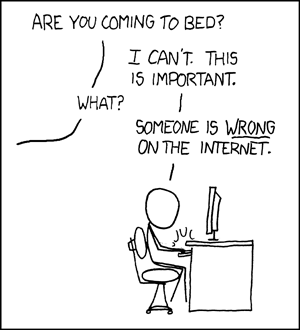
\includegraphics[height=.6\textheight]{fig/duty_calls.png}
\end{figure}
\end{frame}
% - Online discussions as a perfect environment were people encounter very different viewpoints.


\begin{frame}{Online Discussions}
\begin{figure}
	\only<1>{
\includegraphics[width=\textwidth]{fig/reddit-01.png}}
	\only<2>{
\includegraphics[width=\textwidth]{fig/reddit_many.png}}
\end{figure}
\end{frame}

\begin{frame}{The Subreddit \texttt{/r/ChangeMyView}}
\begin{figure}
	\only<1>{
\includegraphics[width=\textwidth]{fig/reddit-02.png}}
	\only<2>{
\includegraphics[width=\textwidth]{fig/reddit-03.png}}
	\only<3>{
\includegraphics[width=\textwidth]{fig/reddit-04.png}}
	\only<4>{
\includegraphics[width=\textwidth]{fig/reddit-05.png}}
	\only<5>{
\includegraphics[width=.95\textwidth]{fig/reddit_screenshot.png}}
\end{figure}
\end{frame}



\section{Empirical Results}


\subsection{Overview}

\begin{frame}{Analyses}
Describe dataset in more detail, include discussion of moral foundations dictionary
\end{frame}

\begin{frame}{Extracting Topics from Text -- Latent Dirichlet Allocation}
\begin{figure}
	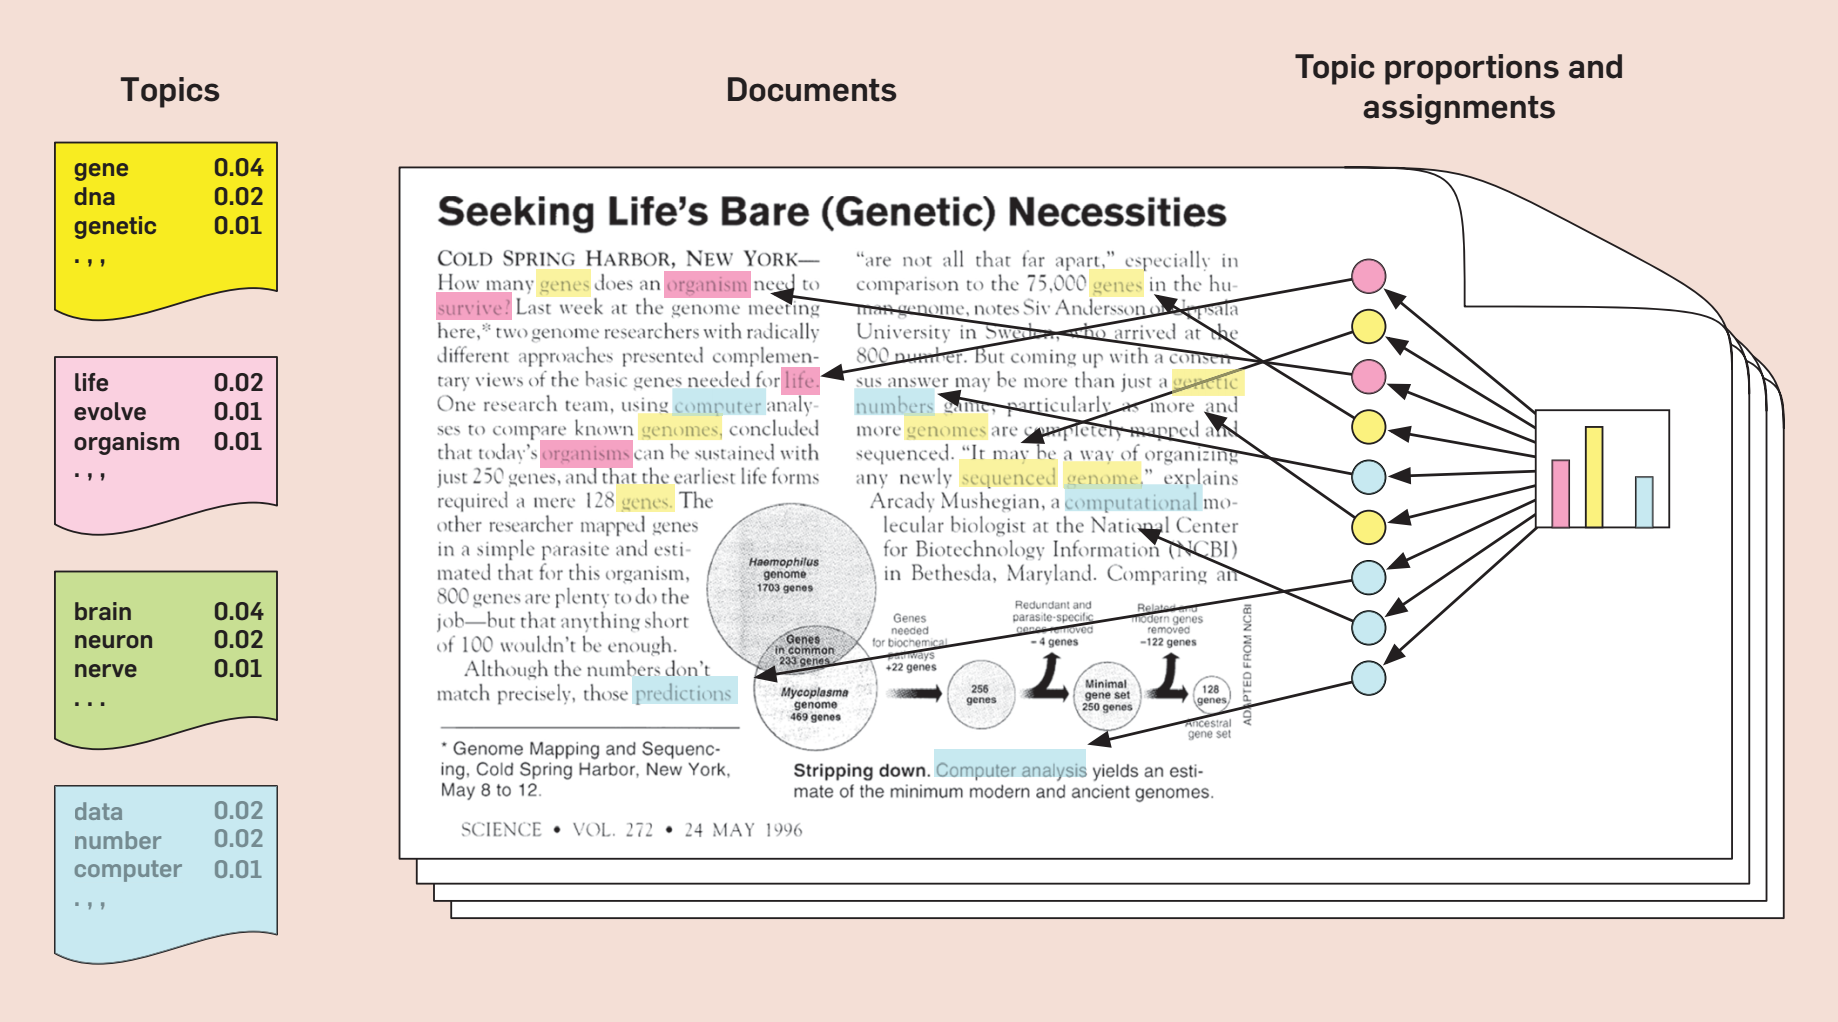
\includegraphics[width=\textwidth]{fig/blei2012probabilistic.png}
\end{figure}
\tiny{\textit{Source:} \cite{blei2012probabilistic}}
\end{frame}

\begin{frame}{Discussion Topics on \texttt{/r/ChangeMyView}}
\begin{figure}
\only<1>{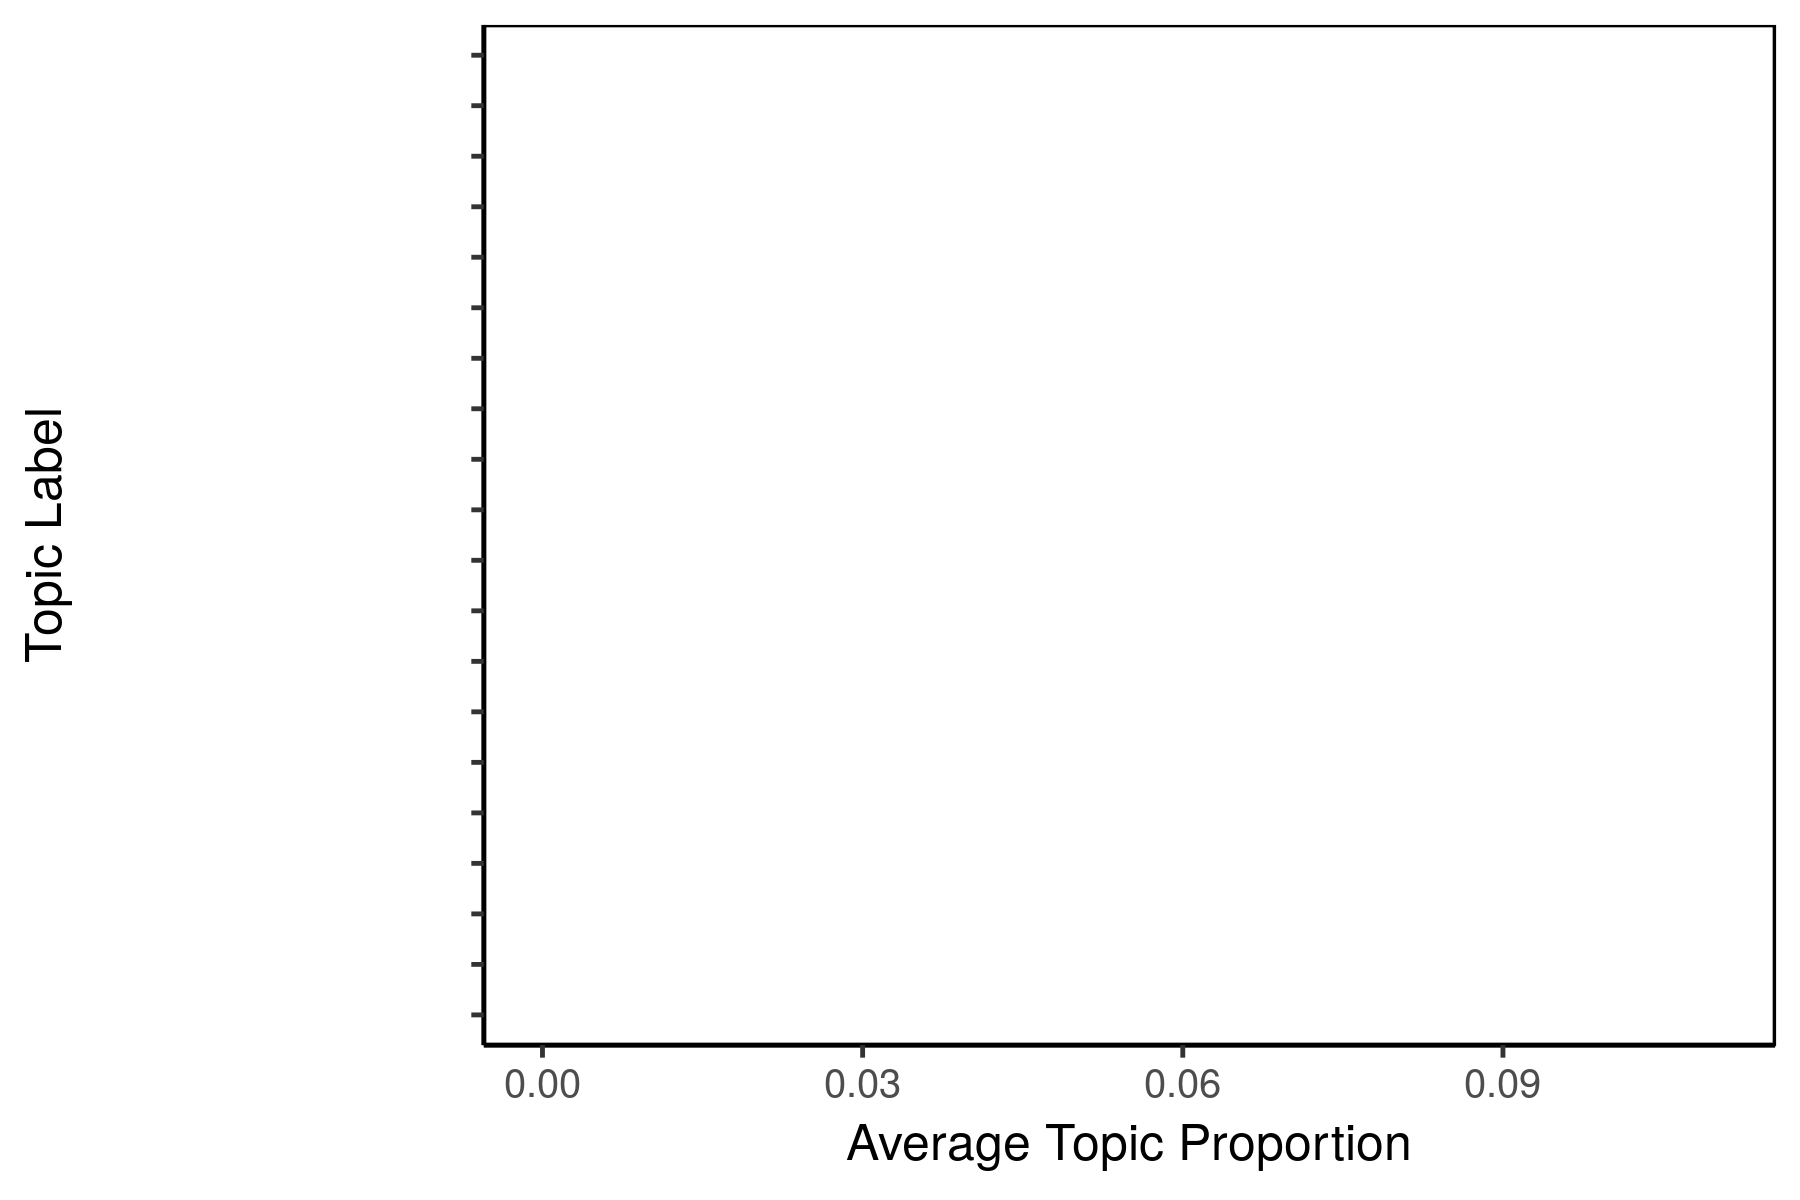
\includegraphics{../calc/fig/topics_00.png}}\only<2>{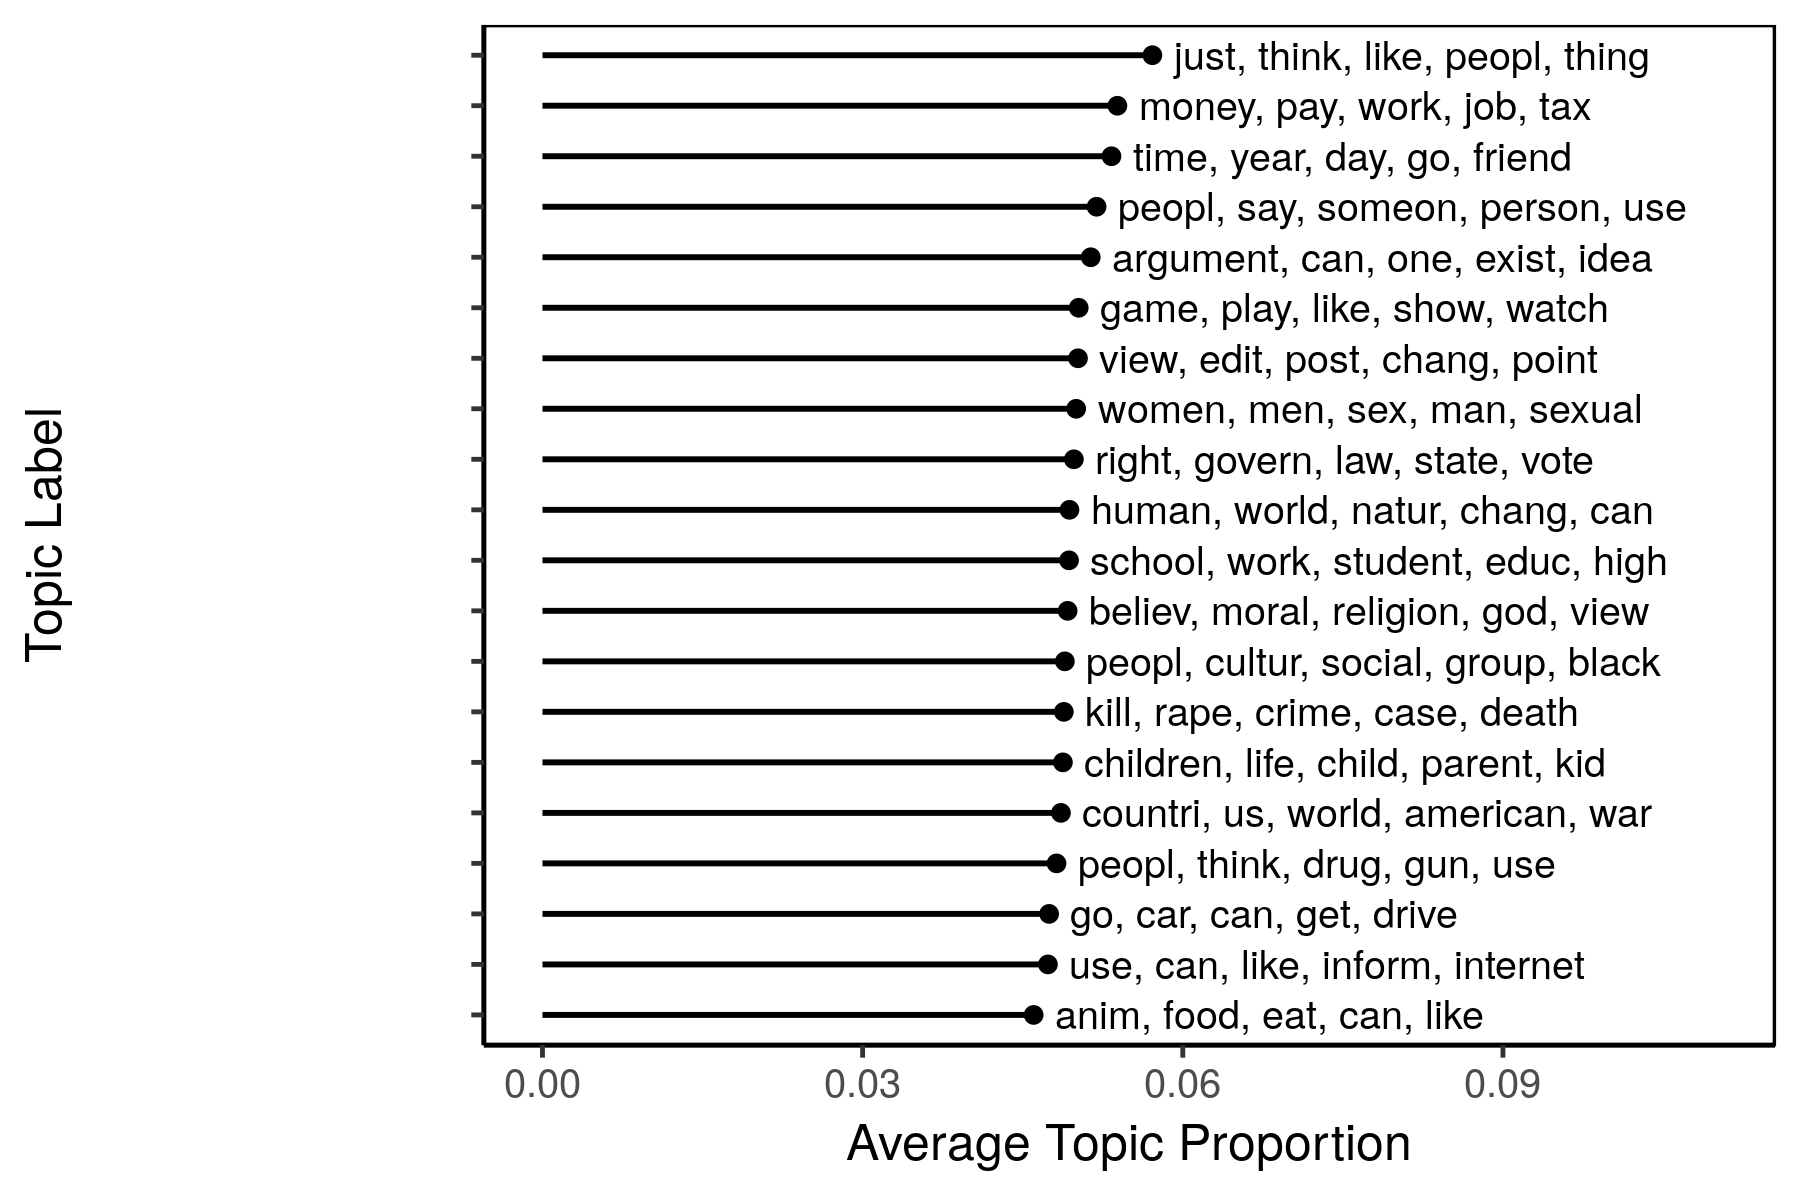
\includegraphics{../calc/fig/topics_01.png}}\only<3>{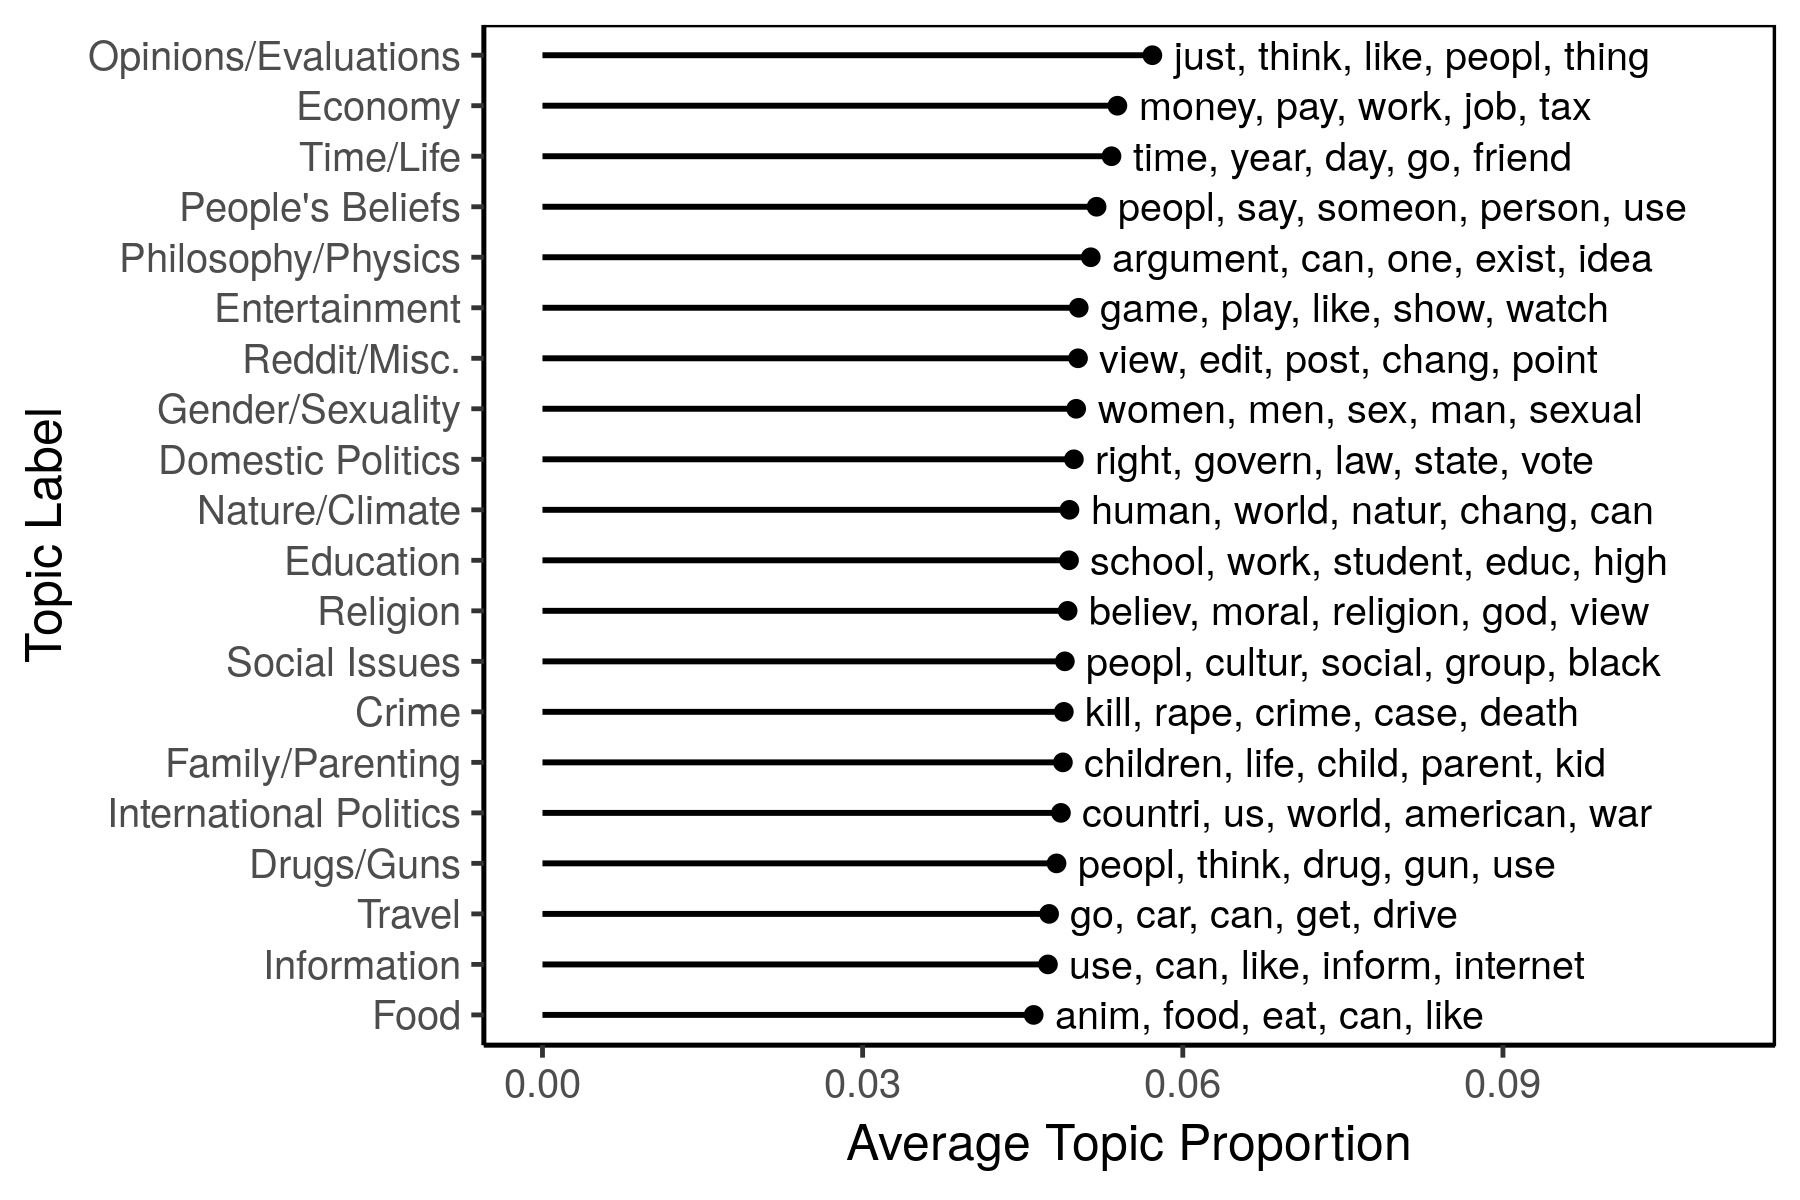
\includegraphics{../calc/fig/topics_02.png}}
\end{figure}
\end{frame}

\begin{frame}{Awarding $\Delta$s on \texttt{/r/ChangeMyView}}
\begin{figure}
\only<1>{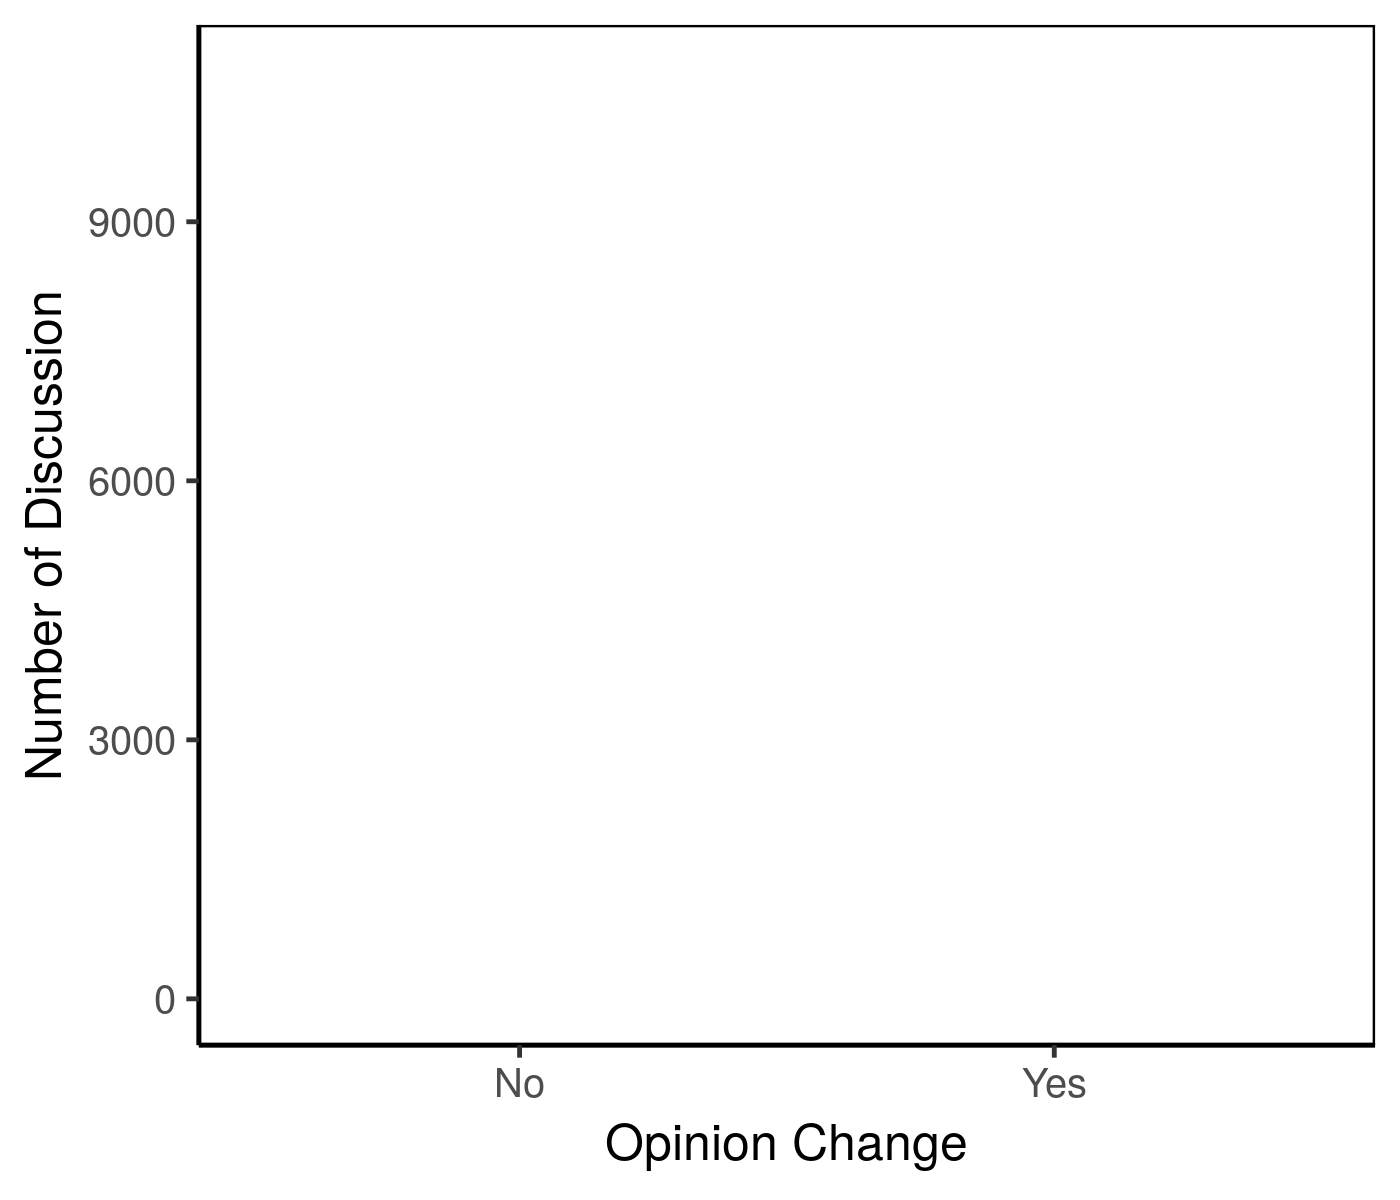
\includegraphics{../calc/fig/delta_empty.png}}\only<2>{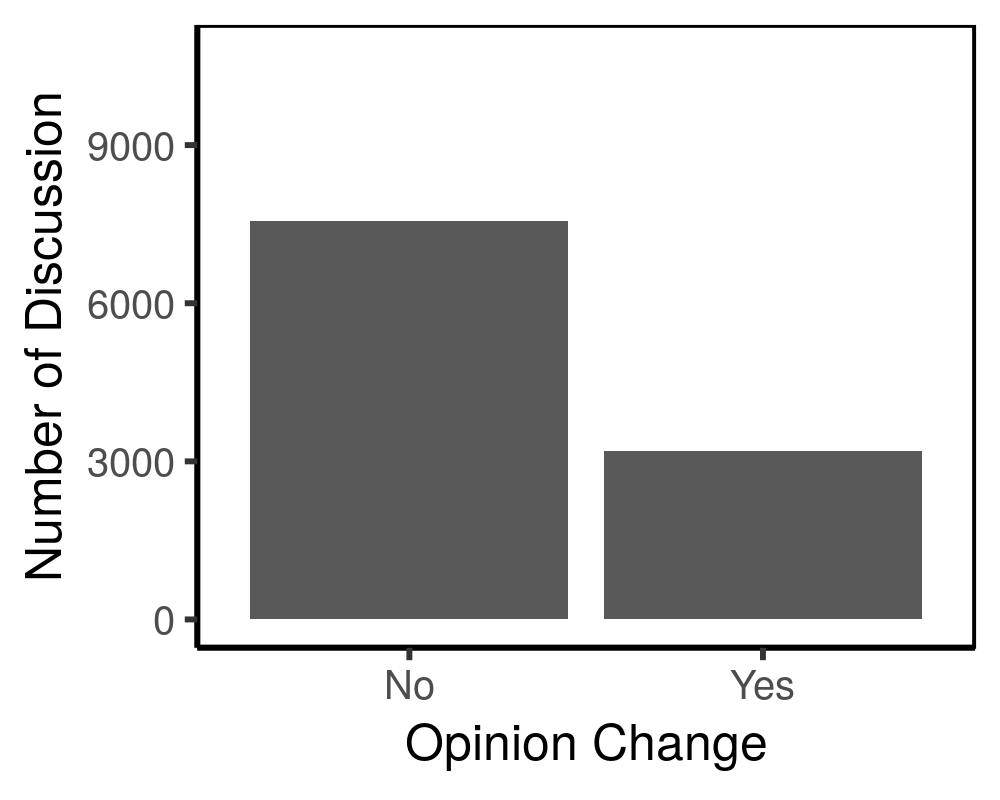
\includegraphics{../calc/fig/delta.png}}
\end{figure}
\end{frame}

% TODO: Add slide on how to measure moral foundations

\begin{frame}{Moral Foundations and Persuadability}
\begin{figure}
	\only<1>{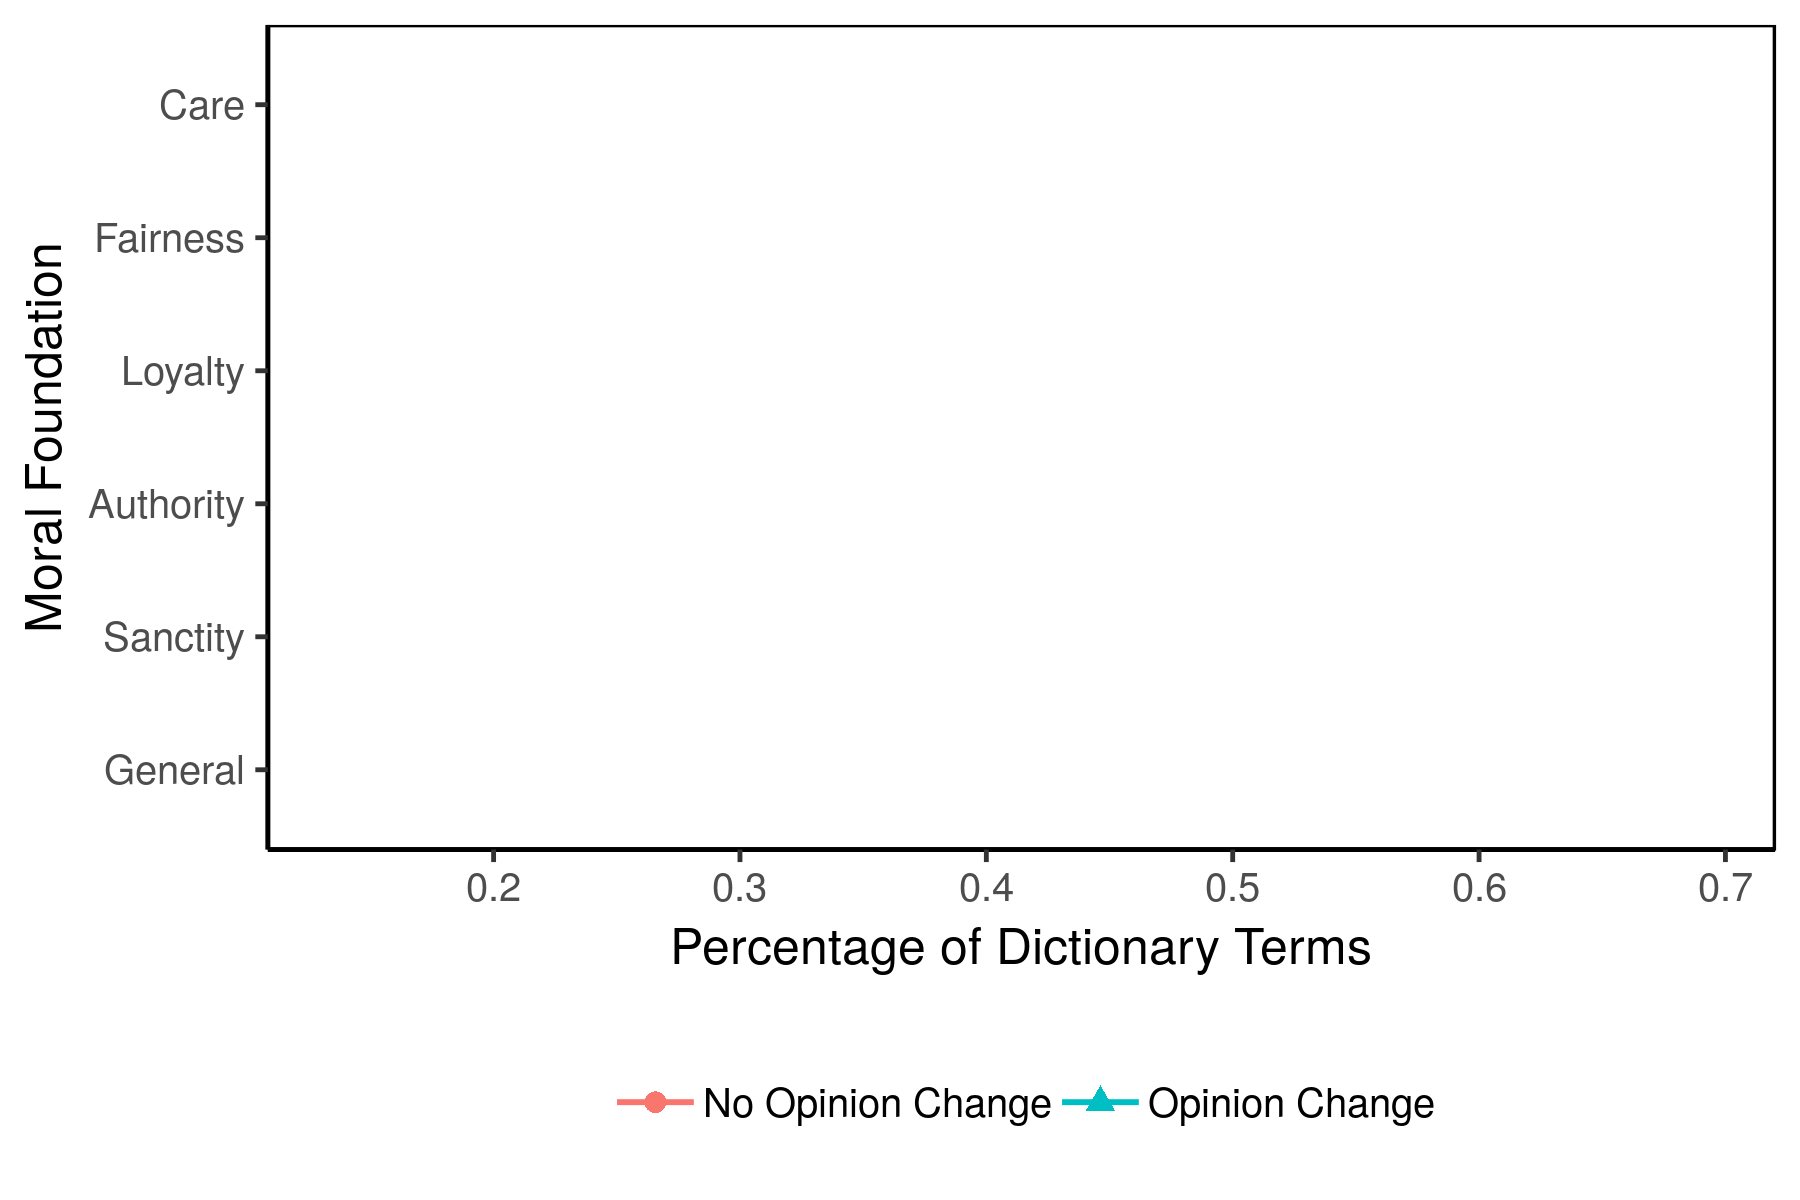
\includegraphics{../calc/fig/persuadability_empty.png}}\only<2>{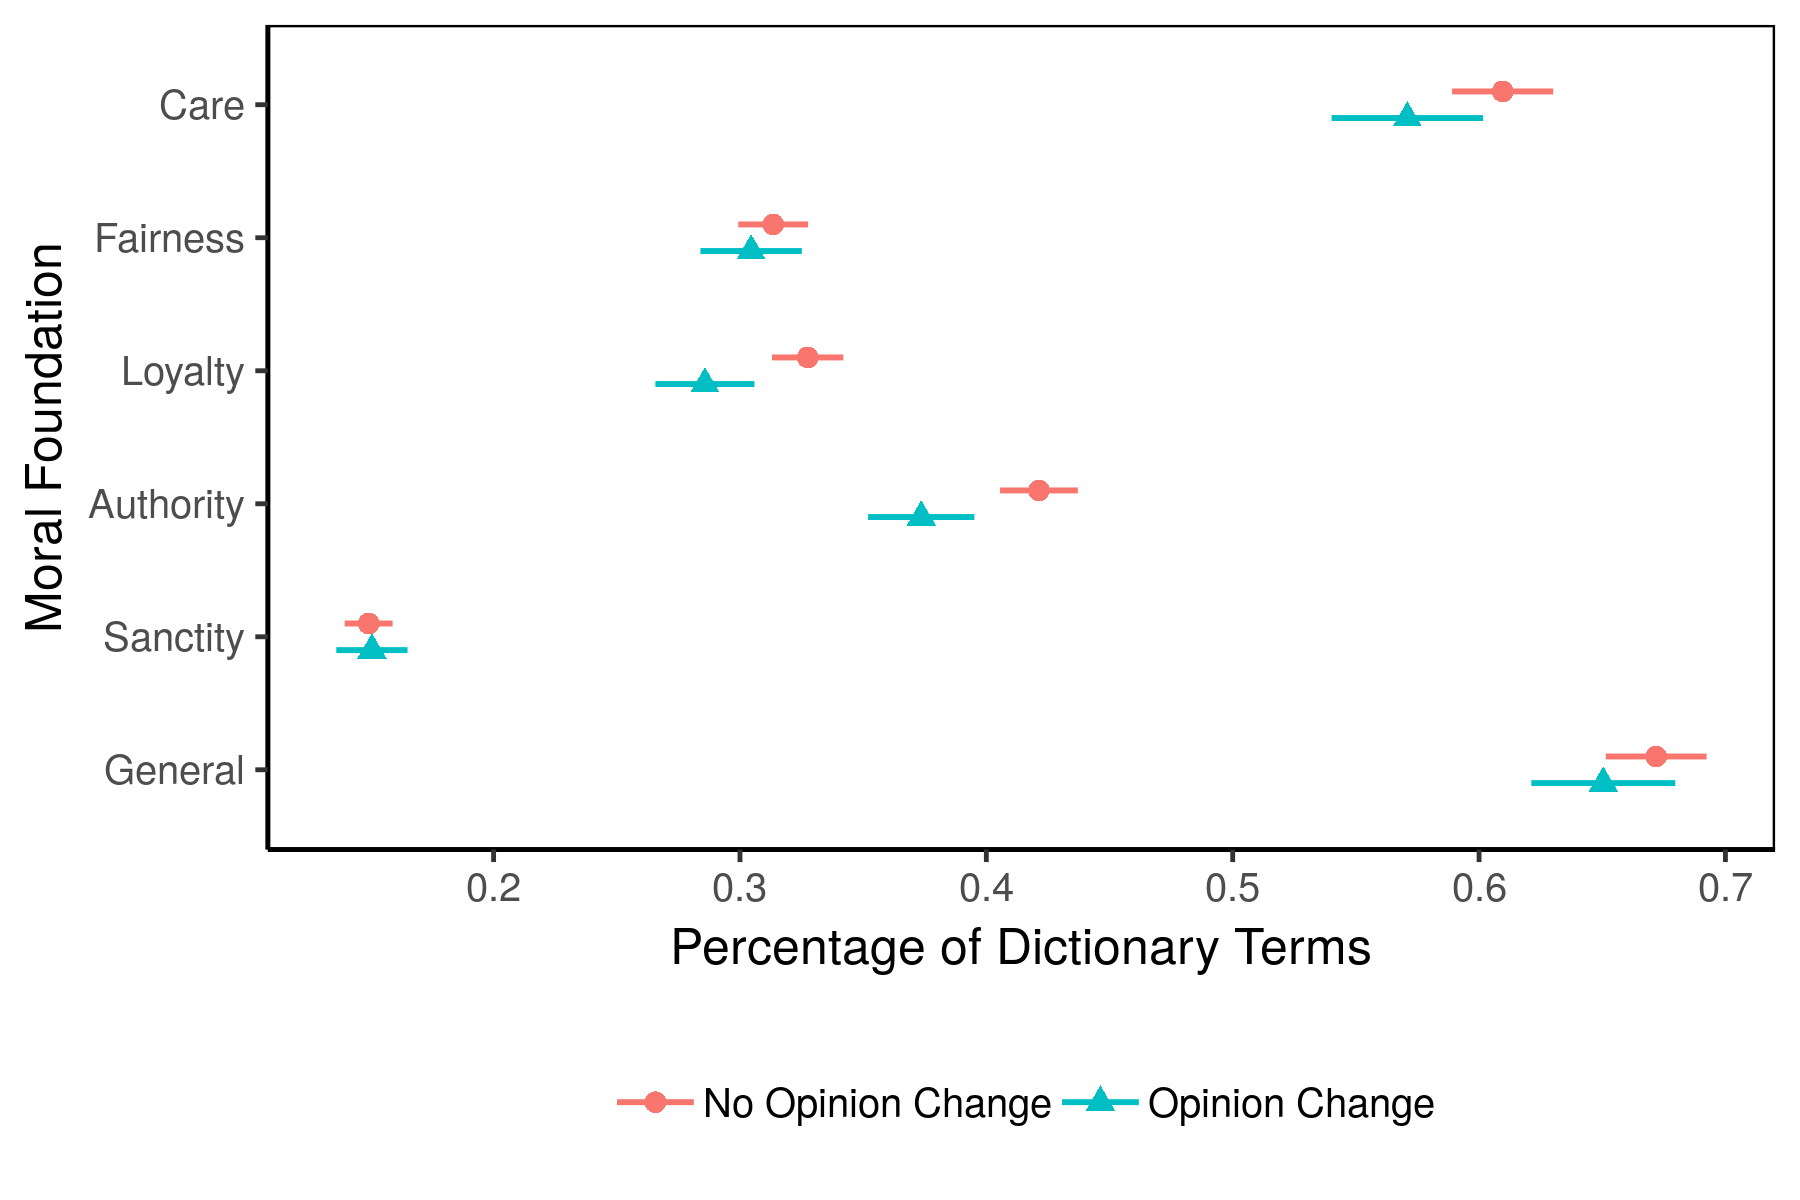
\includegraphics{../calc/fig/persuadability.png}}
\end{figure}
\end{frame}

\begin{frame}{The Subreddit \texttt{/r/ChangeMyView}}
\begin{figure}
	\only<1>{
\includegraphics[width=\textwidth]{fig/reddit-05.png}}
	\only<2>{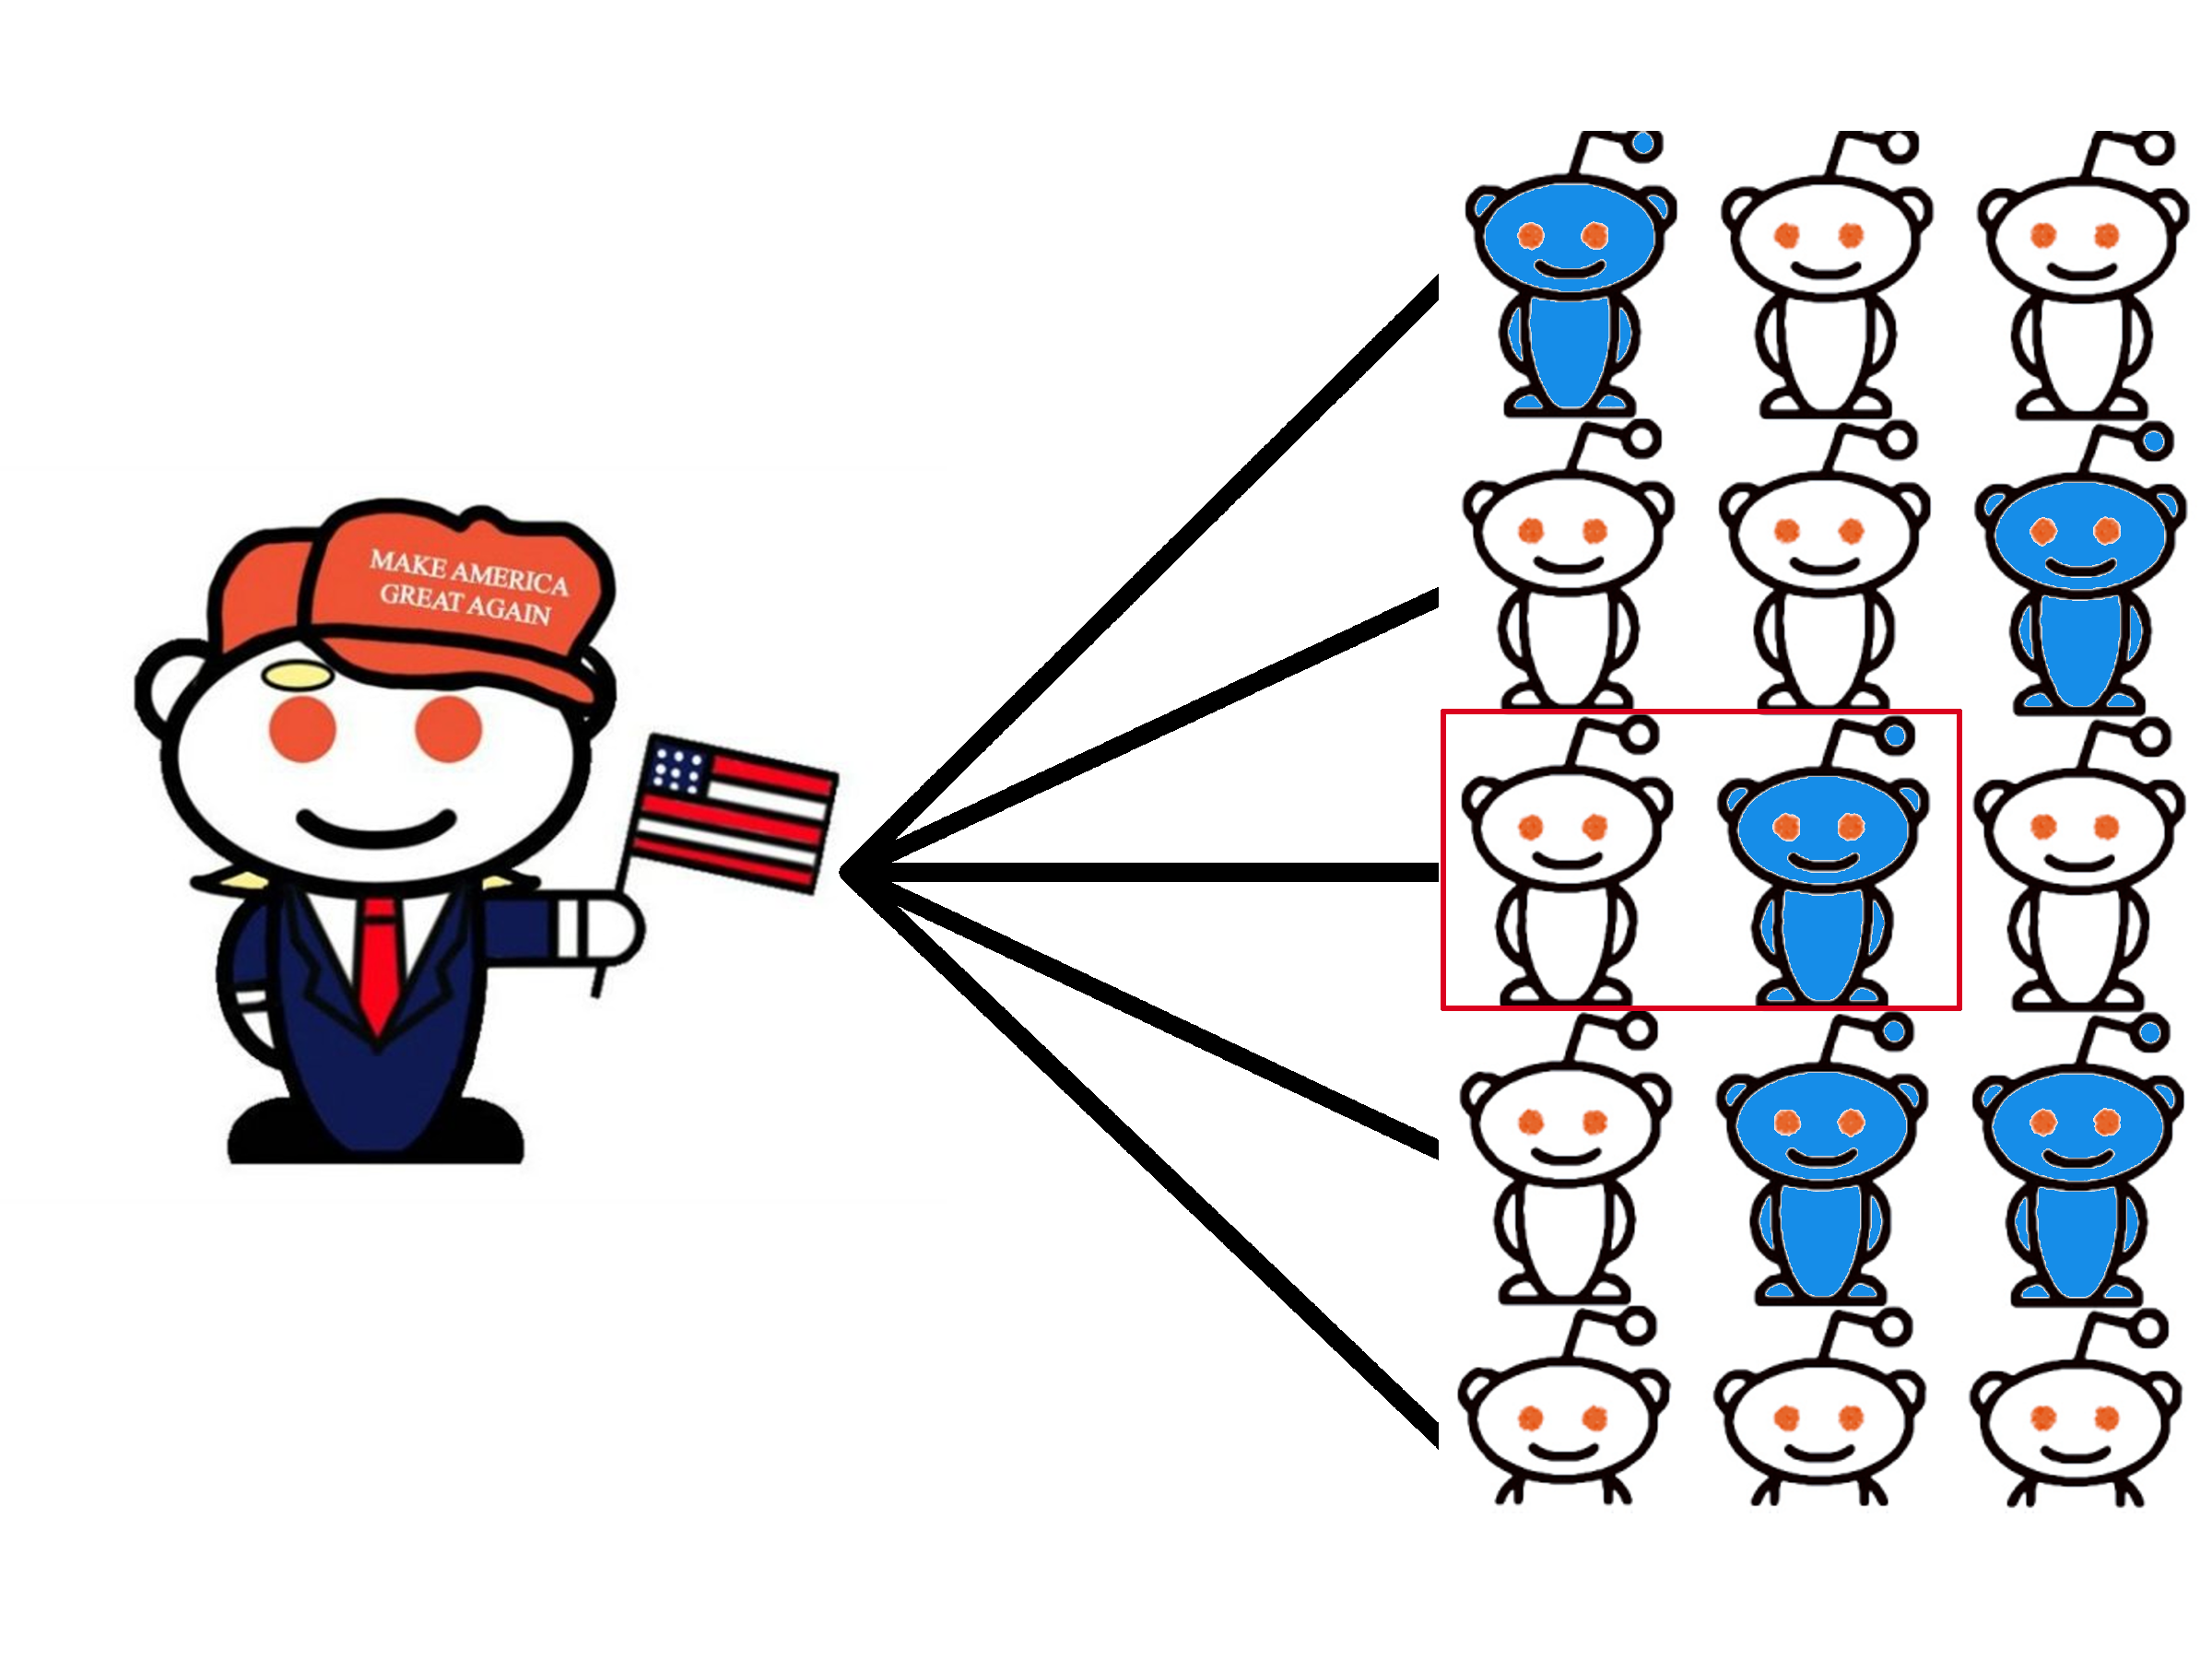
\includegraphics[width=\textwidth]{fig/reddit-06.png}}
\end{figure}
\end{frame}

\begin{frame}{Matching Similar Arguments}\centering
\begin{equation*}
\text{Jaccard}(B_\Delta,B_{\neg\Delta})=\dfrac{|B_\Delta\cap B_{\neg\Delta}|}{|B_\Delta\cup B_{\neg\Delta}|}
\end{equation*}
\vspace{2em}\\
\large{\emph{Question:}\\Which of two lexically similar arguments is the successful one?}
\end{frame}

\begin{frame}{Moral Appeals are Futile}
\begin{figure}
	\only<1>{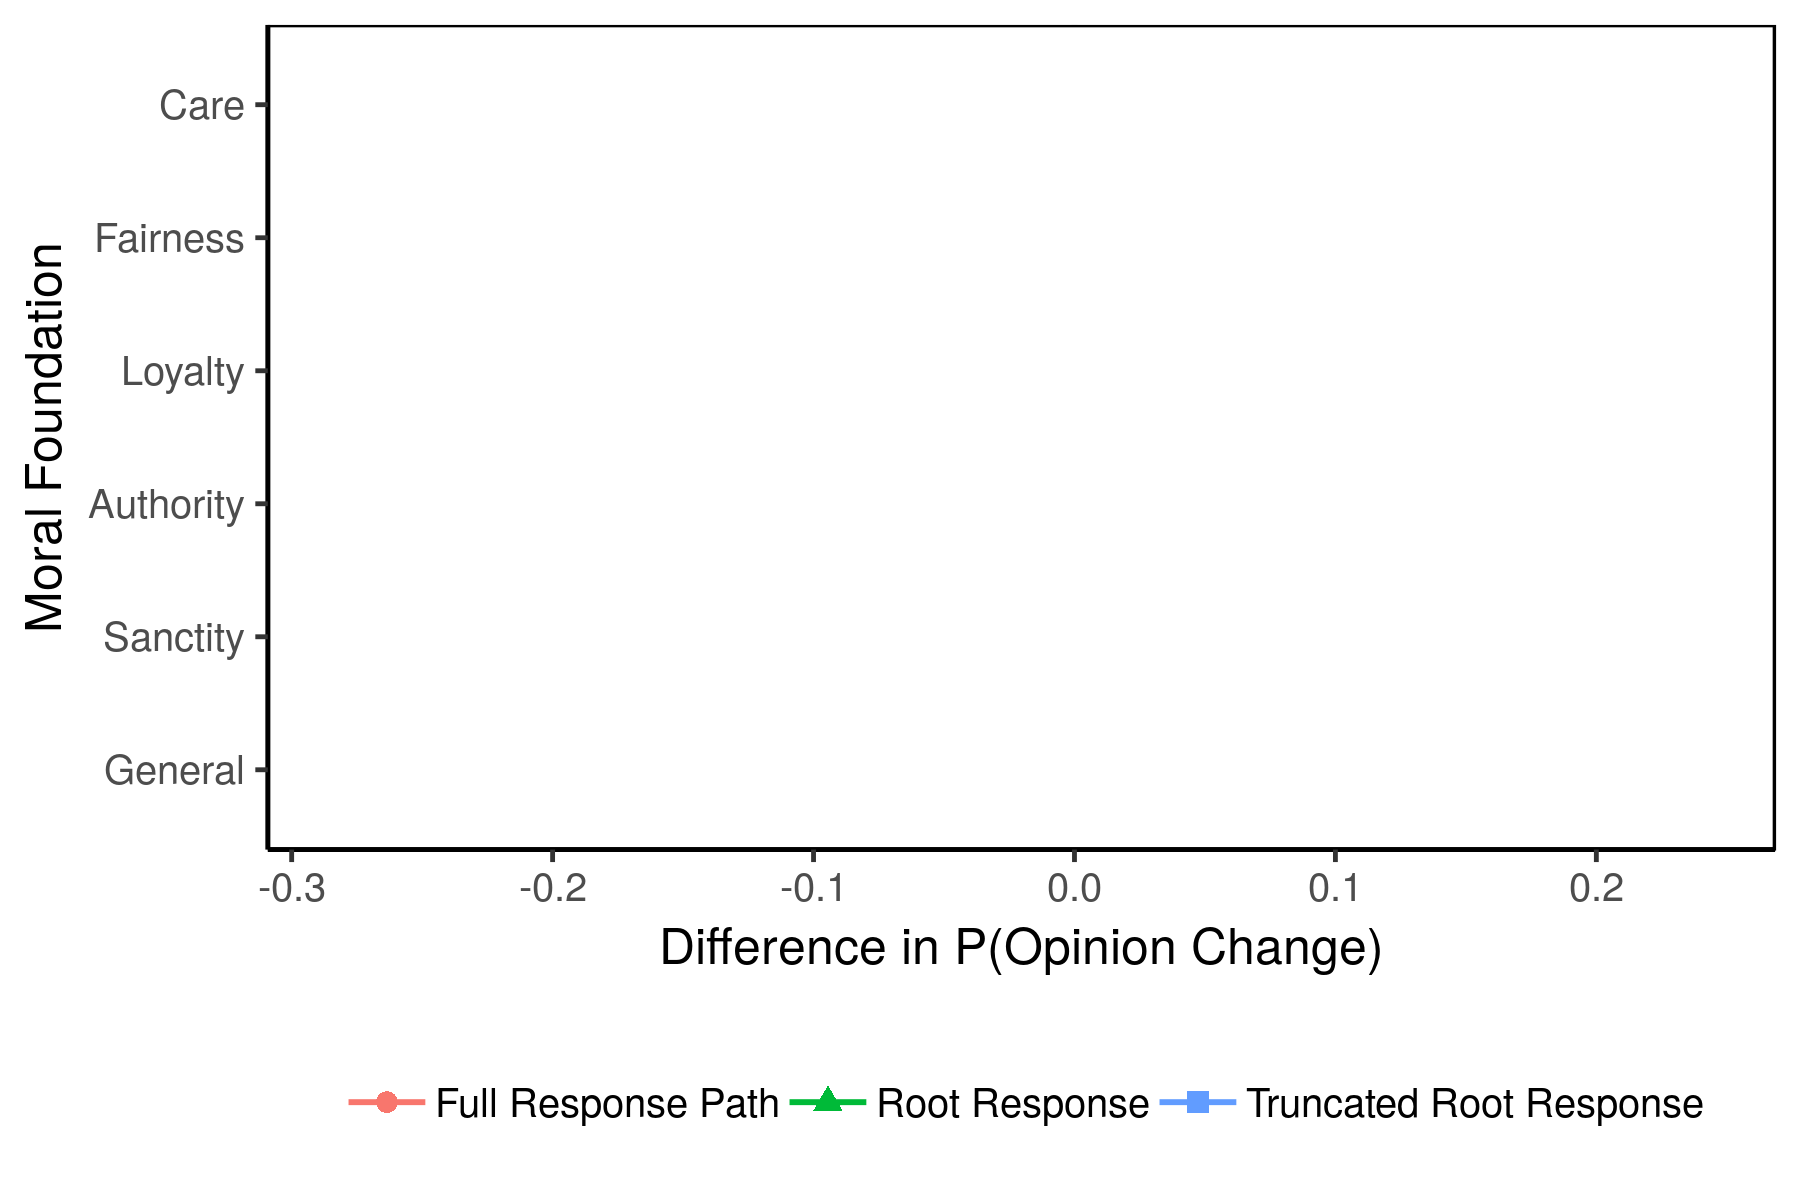
\includegraphics{../calc/fig/logit_persuasiveness_empty.png}}\only<2>{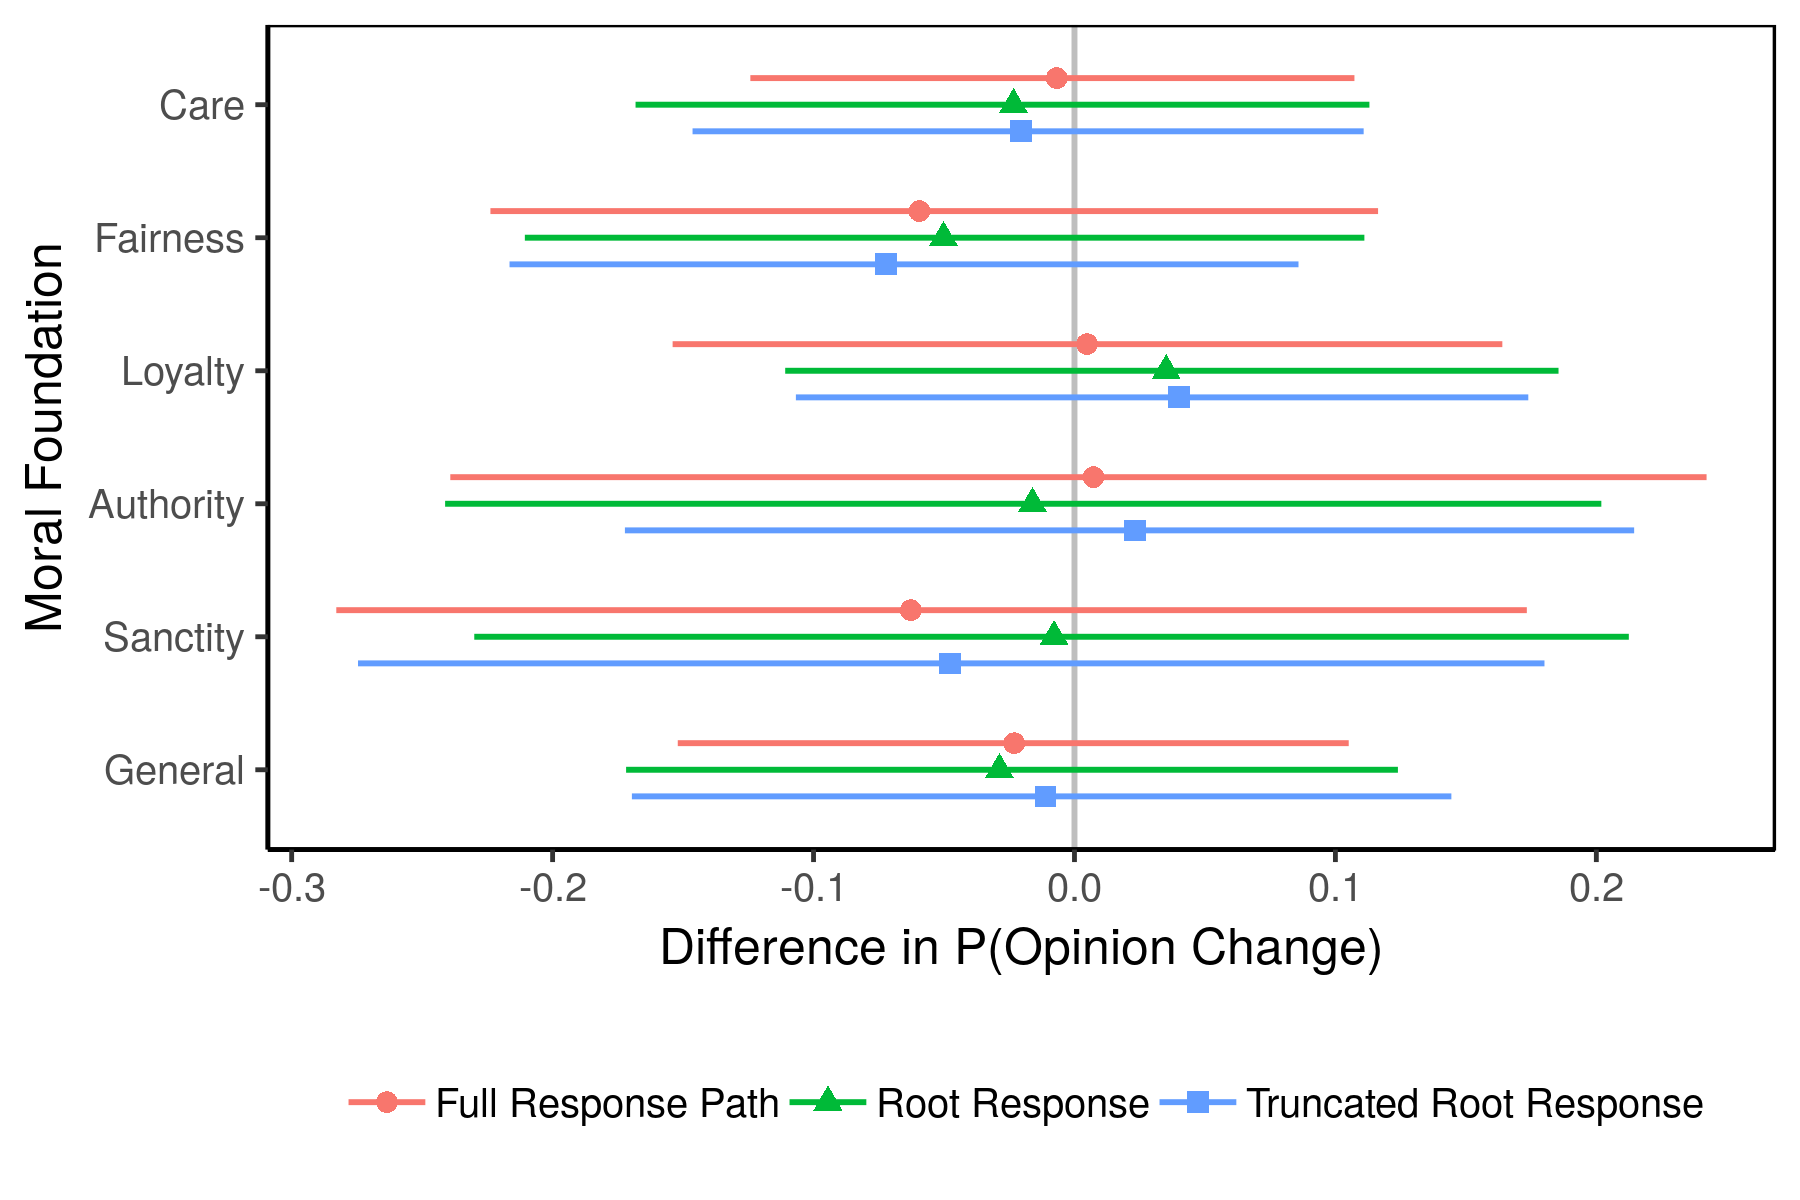
\includegraphics{../calc/fig/logit_persuasiveness.png}}
\end{figure}
\end{frame}

\begin{frame}{Measuring Moral Congruence}\centering
\begin{equation*}
\text{MFT Congruence}=\dfrac{\vec{a}\cdot \vec{b}}{||\vec{a}||\hspace{.2em}||\vec{b}||}
\end{equation*}
\vspace{2em}\\
\large{\emph{Basic Approach:}\\Measure the cosine similarity in dictionary counts between opening statements and counterarguments}
\end{frame}

\begin{frame}{Measuring Moral Congruence}
\begin{figure}
	\only<1>{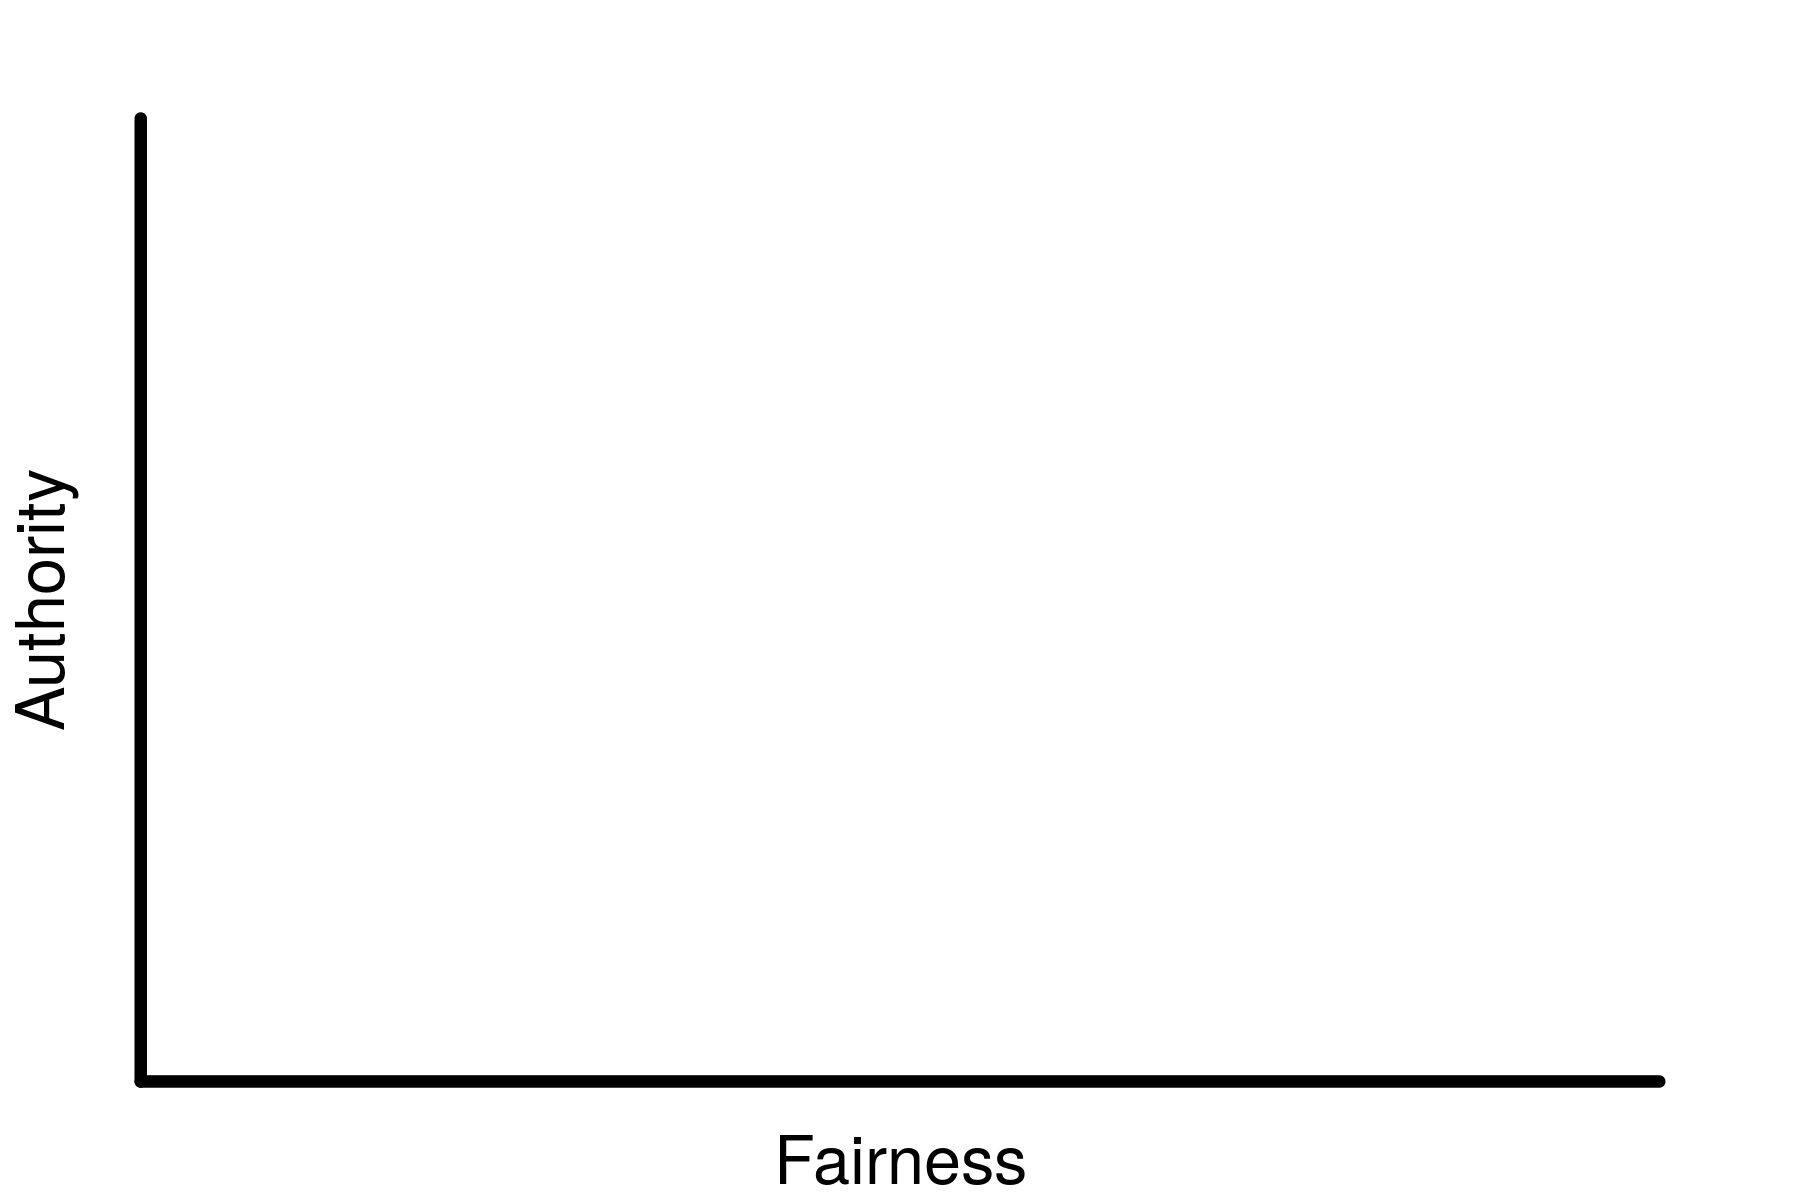
\includegraphics{../calc/fig/cosine_illu0.png}}\only<2>{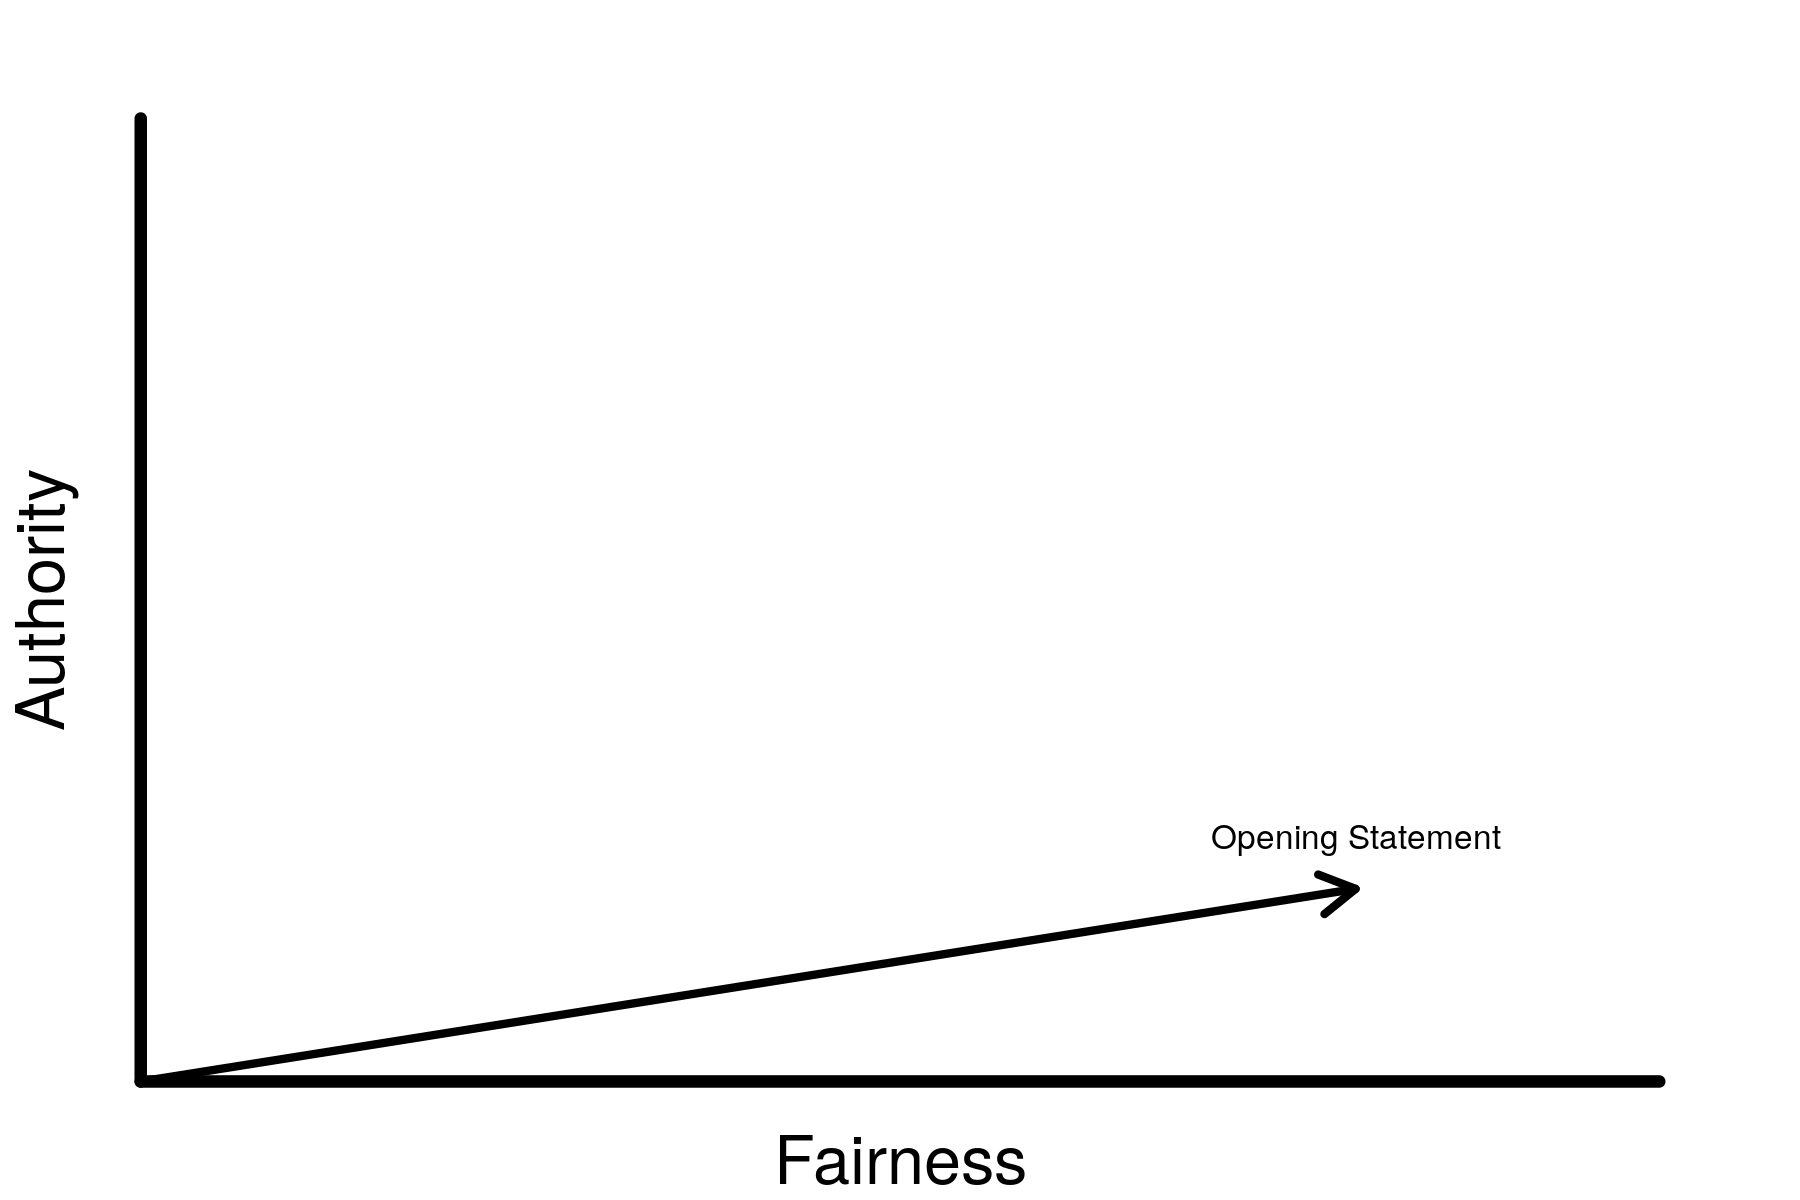
\includegraphics{../calc/fig/cosine_illu1.png}}\only<3>{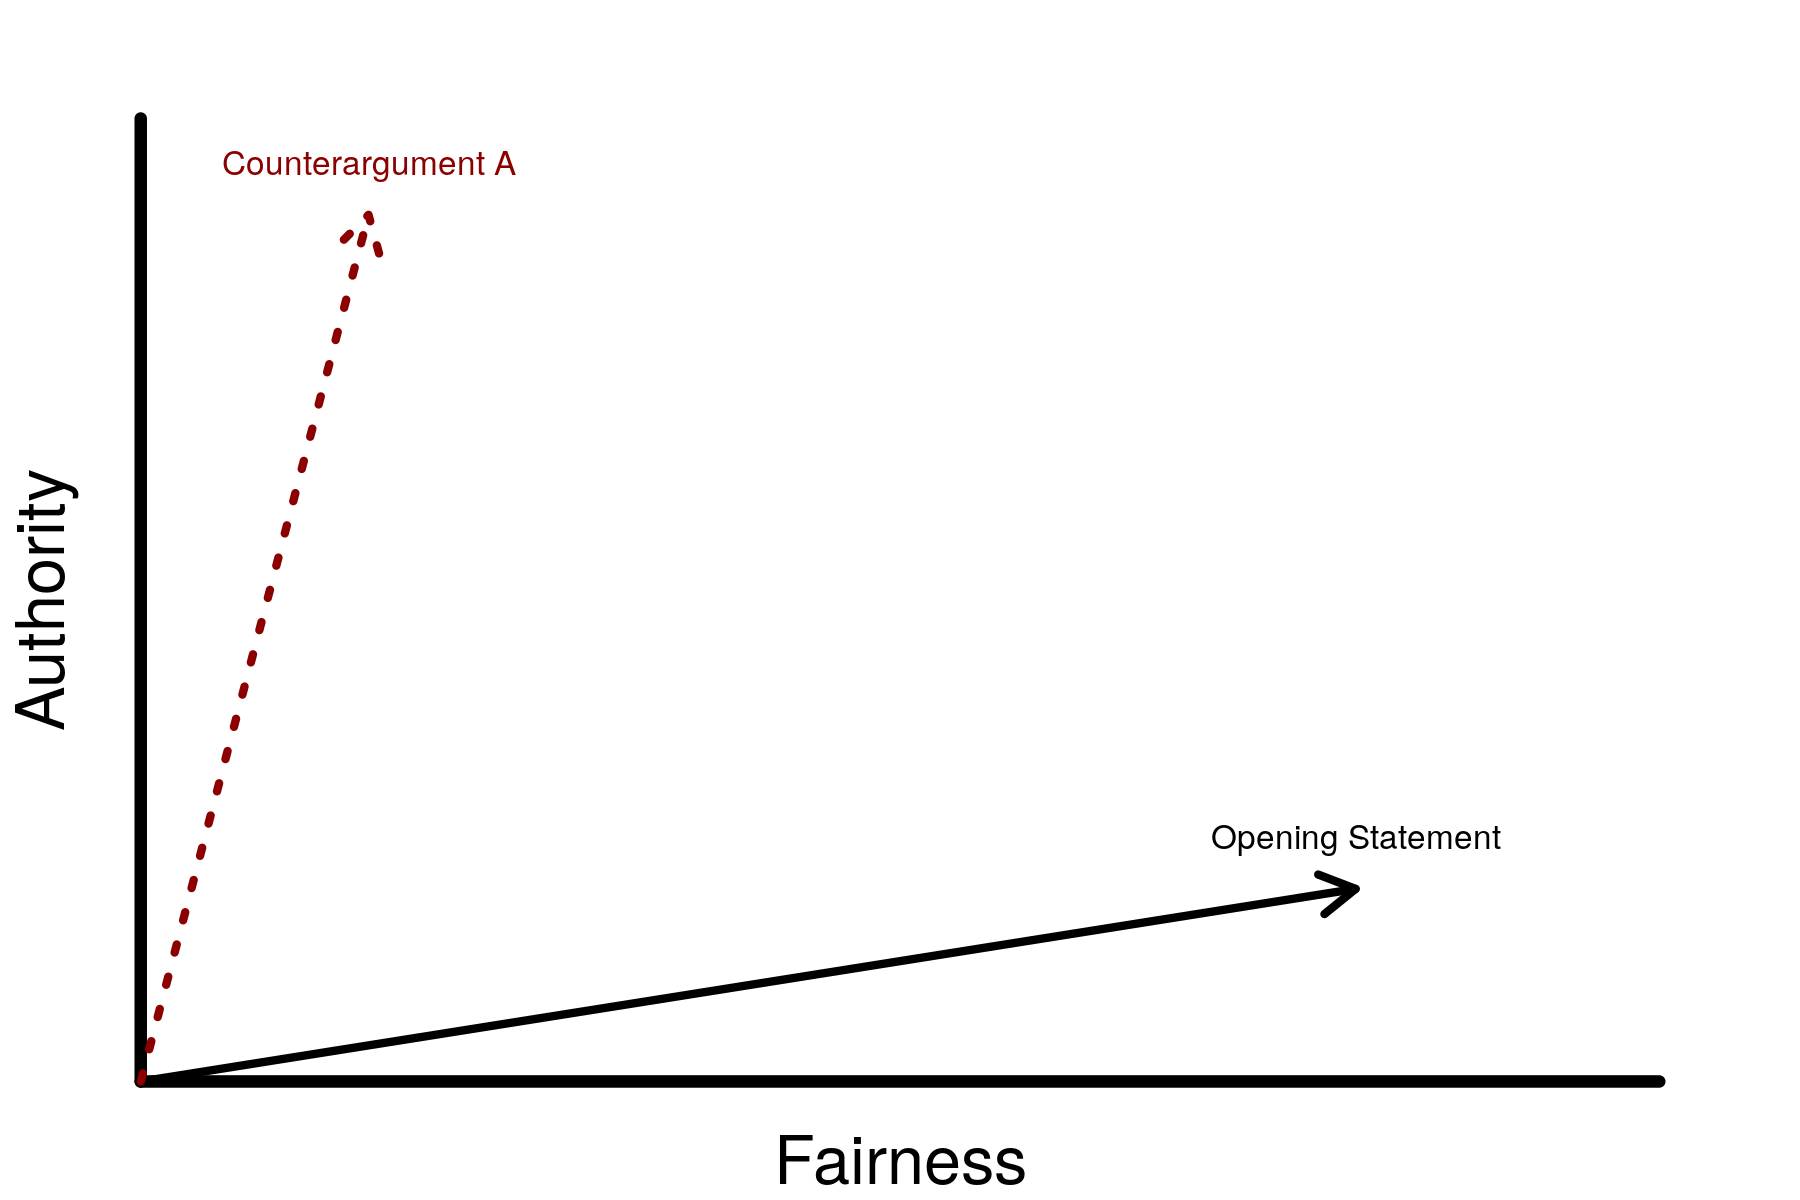
\includegraphics{../calc/fig/cosine_illu2.png}}\only<4>{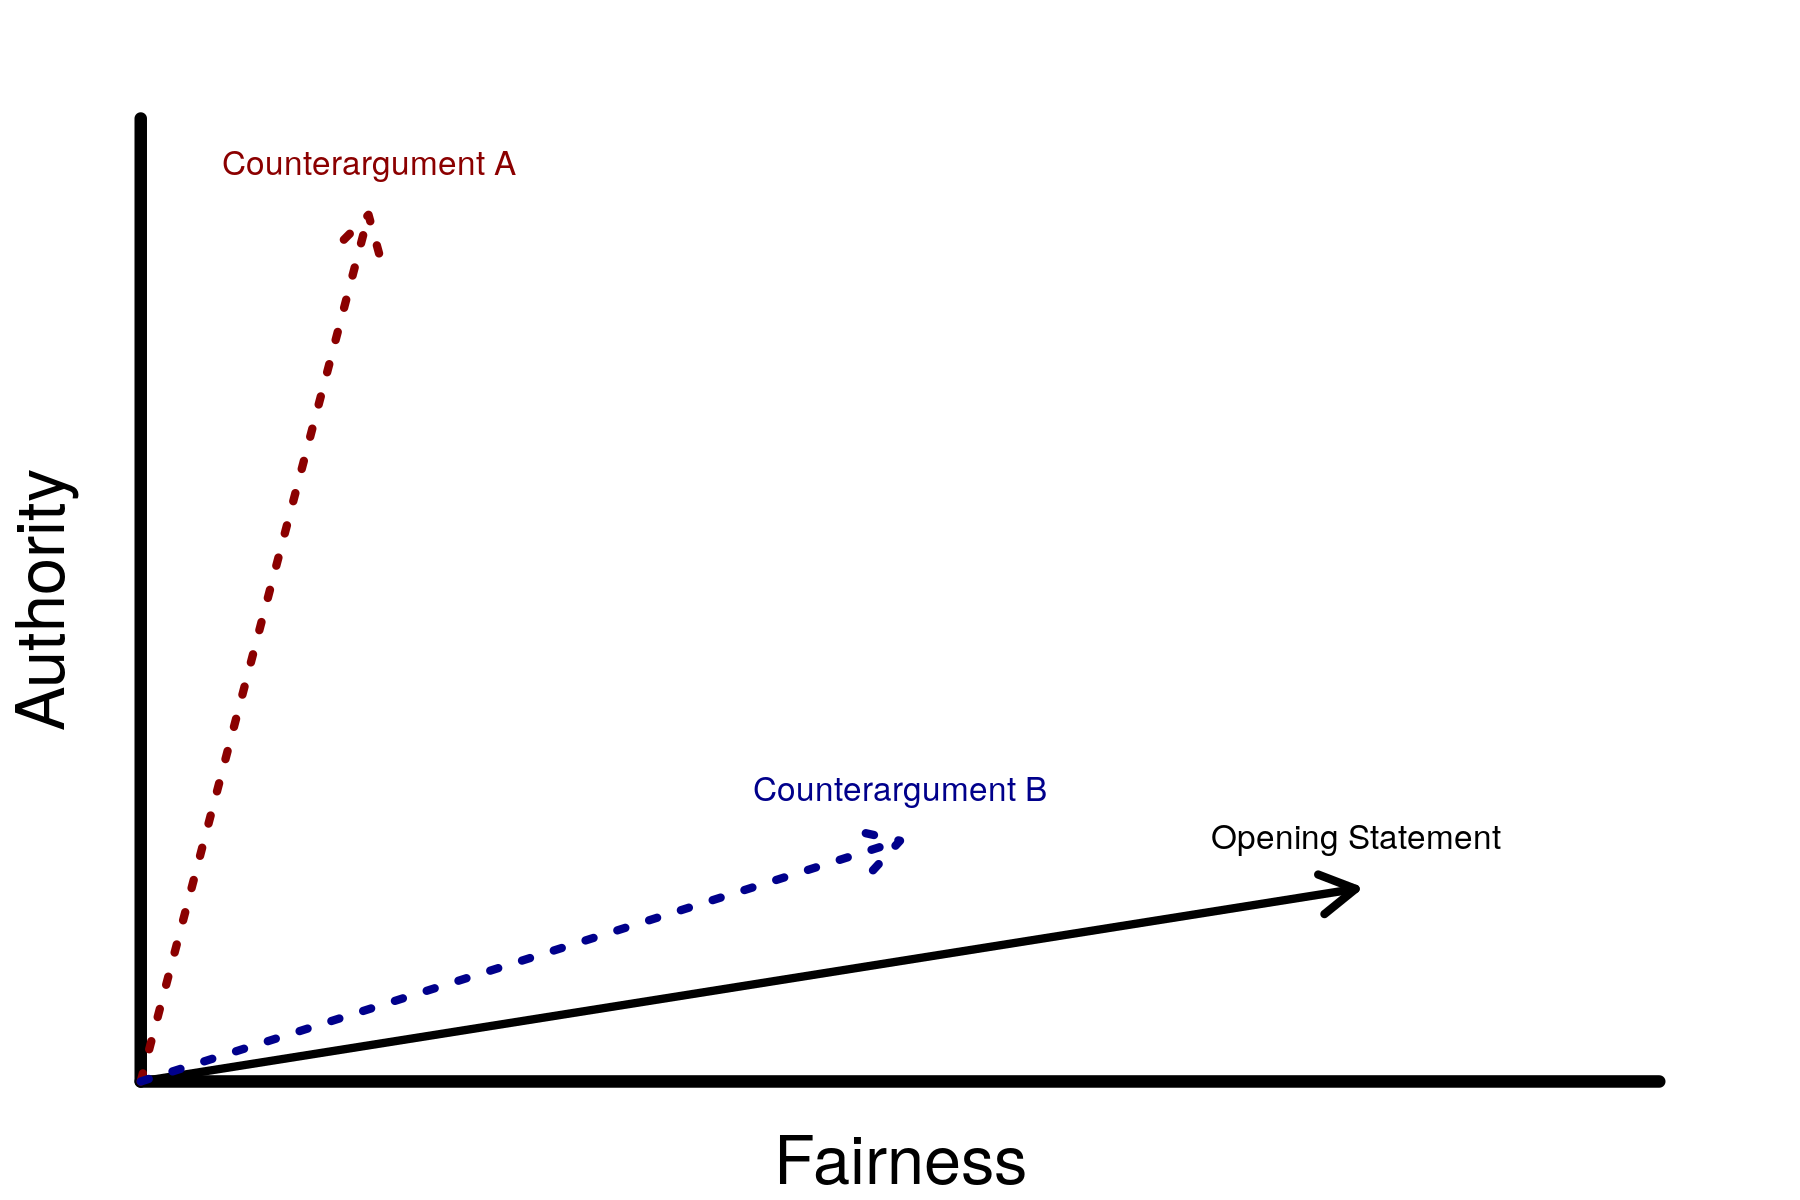
\includegraphics{../calc/fig/cosine_illu3.png}}
\end{figure}
\end{frame}

\begin{frame}{Speaking the Same Moral Language is Effective}\centering
\begin{figure}
\only<1>{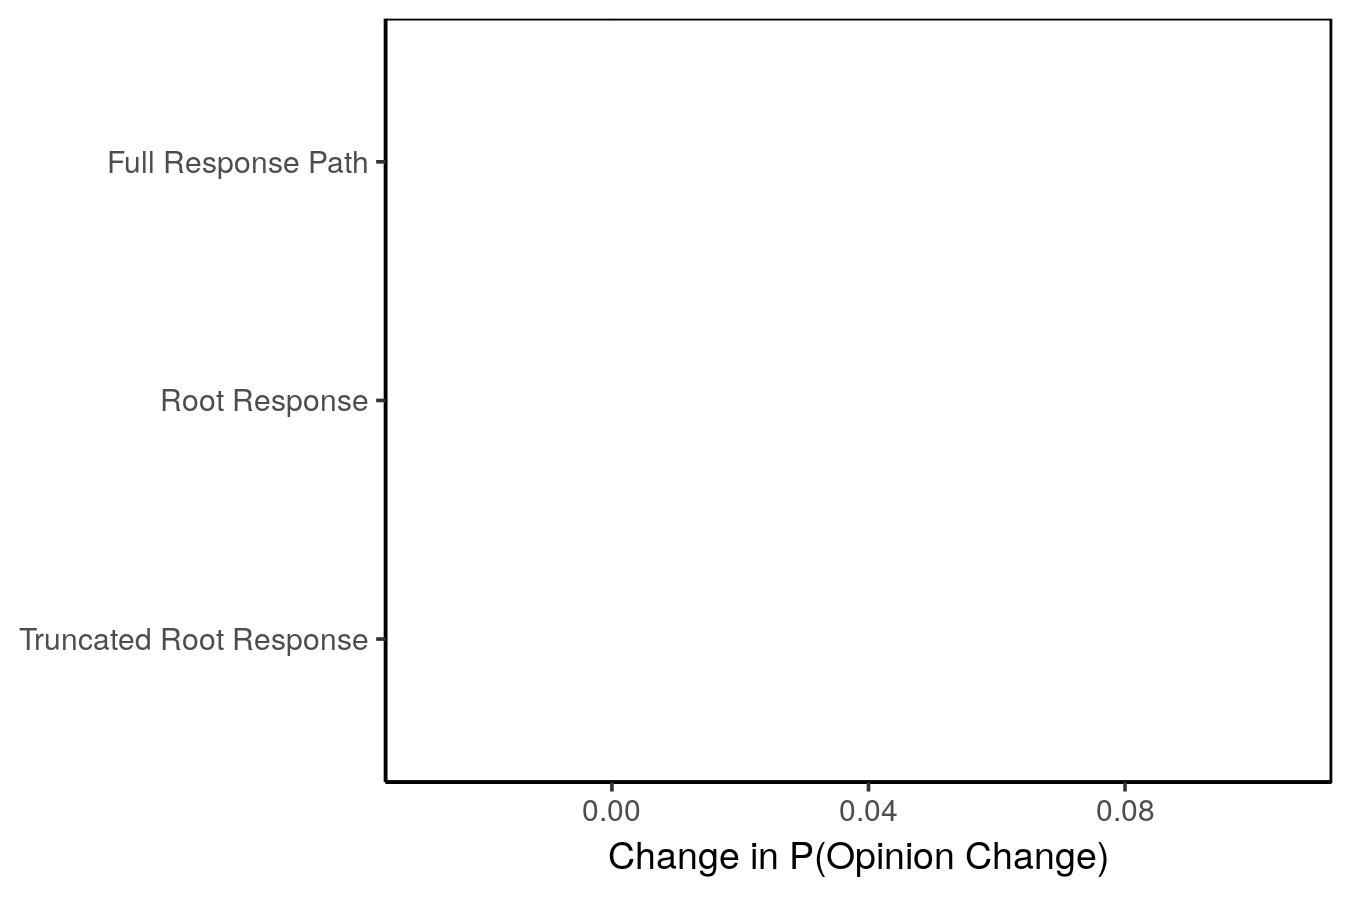
\includegraphics{../calc/fig/logit_cosine_empty.png}}\only<2>{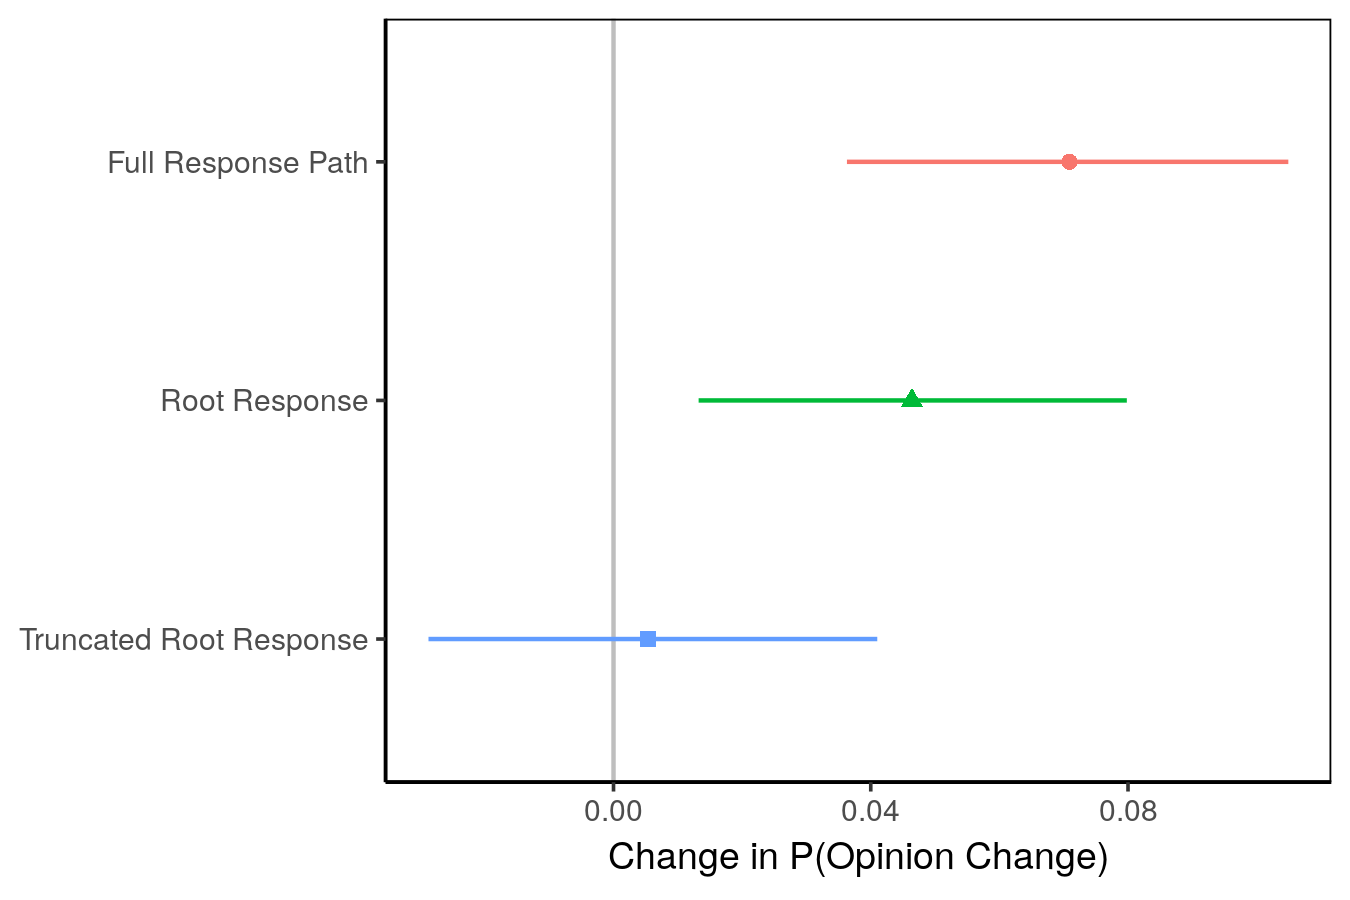
\includegraphics{../calc/fig/logit_cosine.png}}
\end{figure}
\end{frame}


\section{Conclusion}

% TODO: Add slide that summarizes theoretical conclusions

\begin{frame}{Conclusion}
\begin{figure}
	
\includegraphics[height=.8\textheight]{fig/bad_opinions.png}
\end{figure}
\end{frame}

\begin{frame}%[allowframebreaks]
\begin{center}
	{\Large \emph{Thank you very much for your attention!}}\\ \vspace{2em}
	Manuscript and code available at:\\
	%\emph{\texttt{https://github.com/pwkraft/mft}}\\
	\emph{\texttt{https://github.com/pwkraft/cmv}}\\ \vspace{2em}
	Comments, questions?\\
	\emph{\faEnvelopeO\hspace{.5em}\texttt{kraftp@uwm.edu}}\\\vspace{2em}
	\emph{\faGlobe\hspace{.5em}\texttt{pwkraft.github.io}}\\
	\emph{\faTwitter\hspace{.5em}\texttt{@patrickwkraft}}\\
\end{center}
\end{frame}

\section*{Content}
\label{sec:main-content}
\begin{frame}%[allowframebreaks]
\frametitle{Content}
\tableofcontents %[hideallsubsections]
\end{frame}

\appendix
\section*{Appendix Content}
\label{sec:appendix-content}
\begin{frame}%[allowframebreaks]
\frametitle{Appendix Content}
\small\tableofcontents %[hideallsubsections]
\end{frame}

\section{Moral Language in Opening Statements that Received a $\Delta$}
\begin{frame}{Moral Language in Opening Statements that Received a $\Delta$}
\begin{figure}
	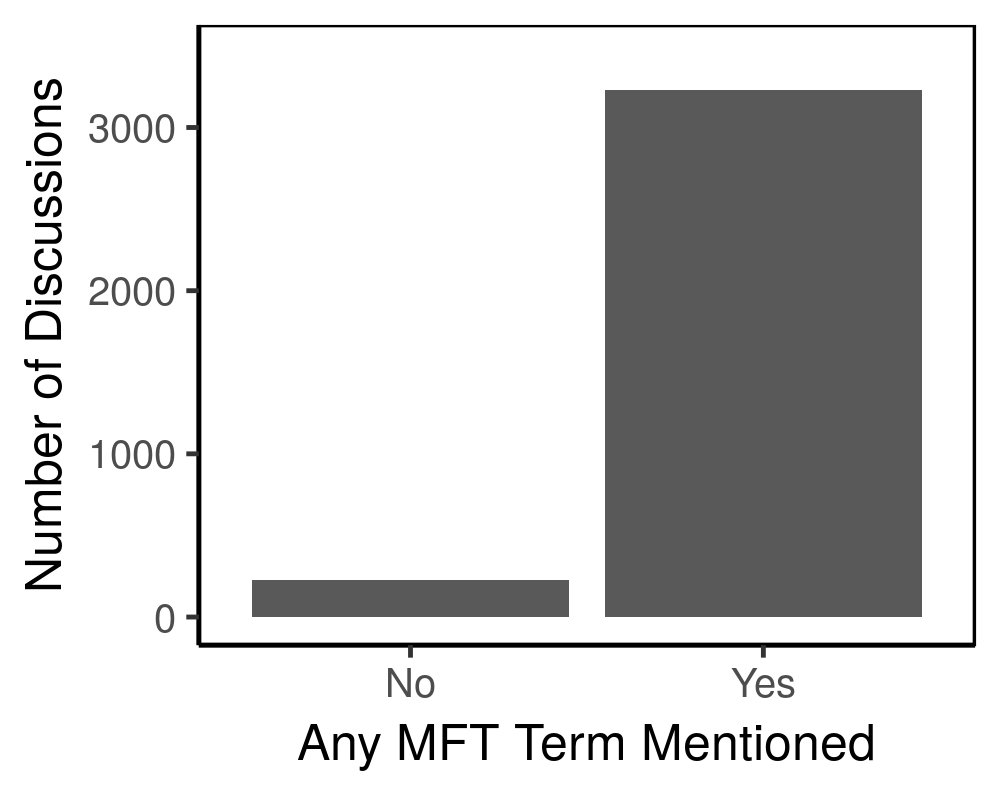
\includegraphics{../calc/fig/mft_op_all.png}
\end{figure}
\end{frame}

\begin{frame}{Moral Language in Opening Statements that Received a $\Delta$}
\begin{figure}
	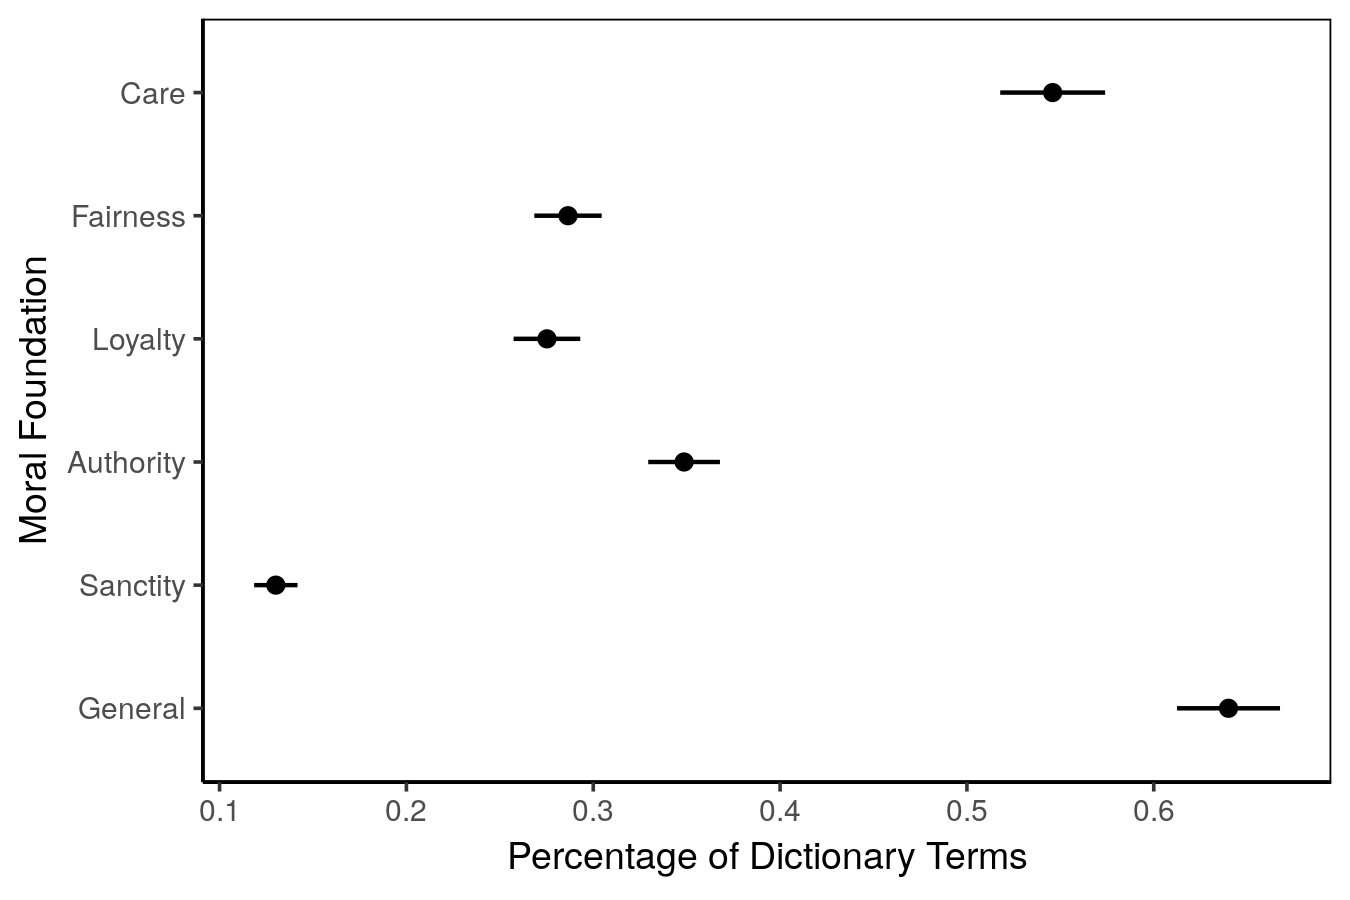
\includegraphics{../calc/fig/mft_op_individual.png}
\end{figure}
\end{frame}

\section{Difference in Response Length}
\begin{frame}{Difference in Response Length}
\begin{figure}
	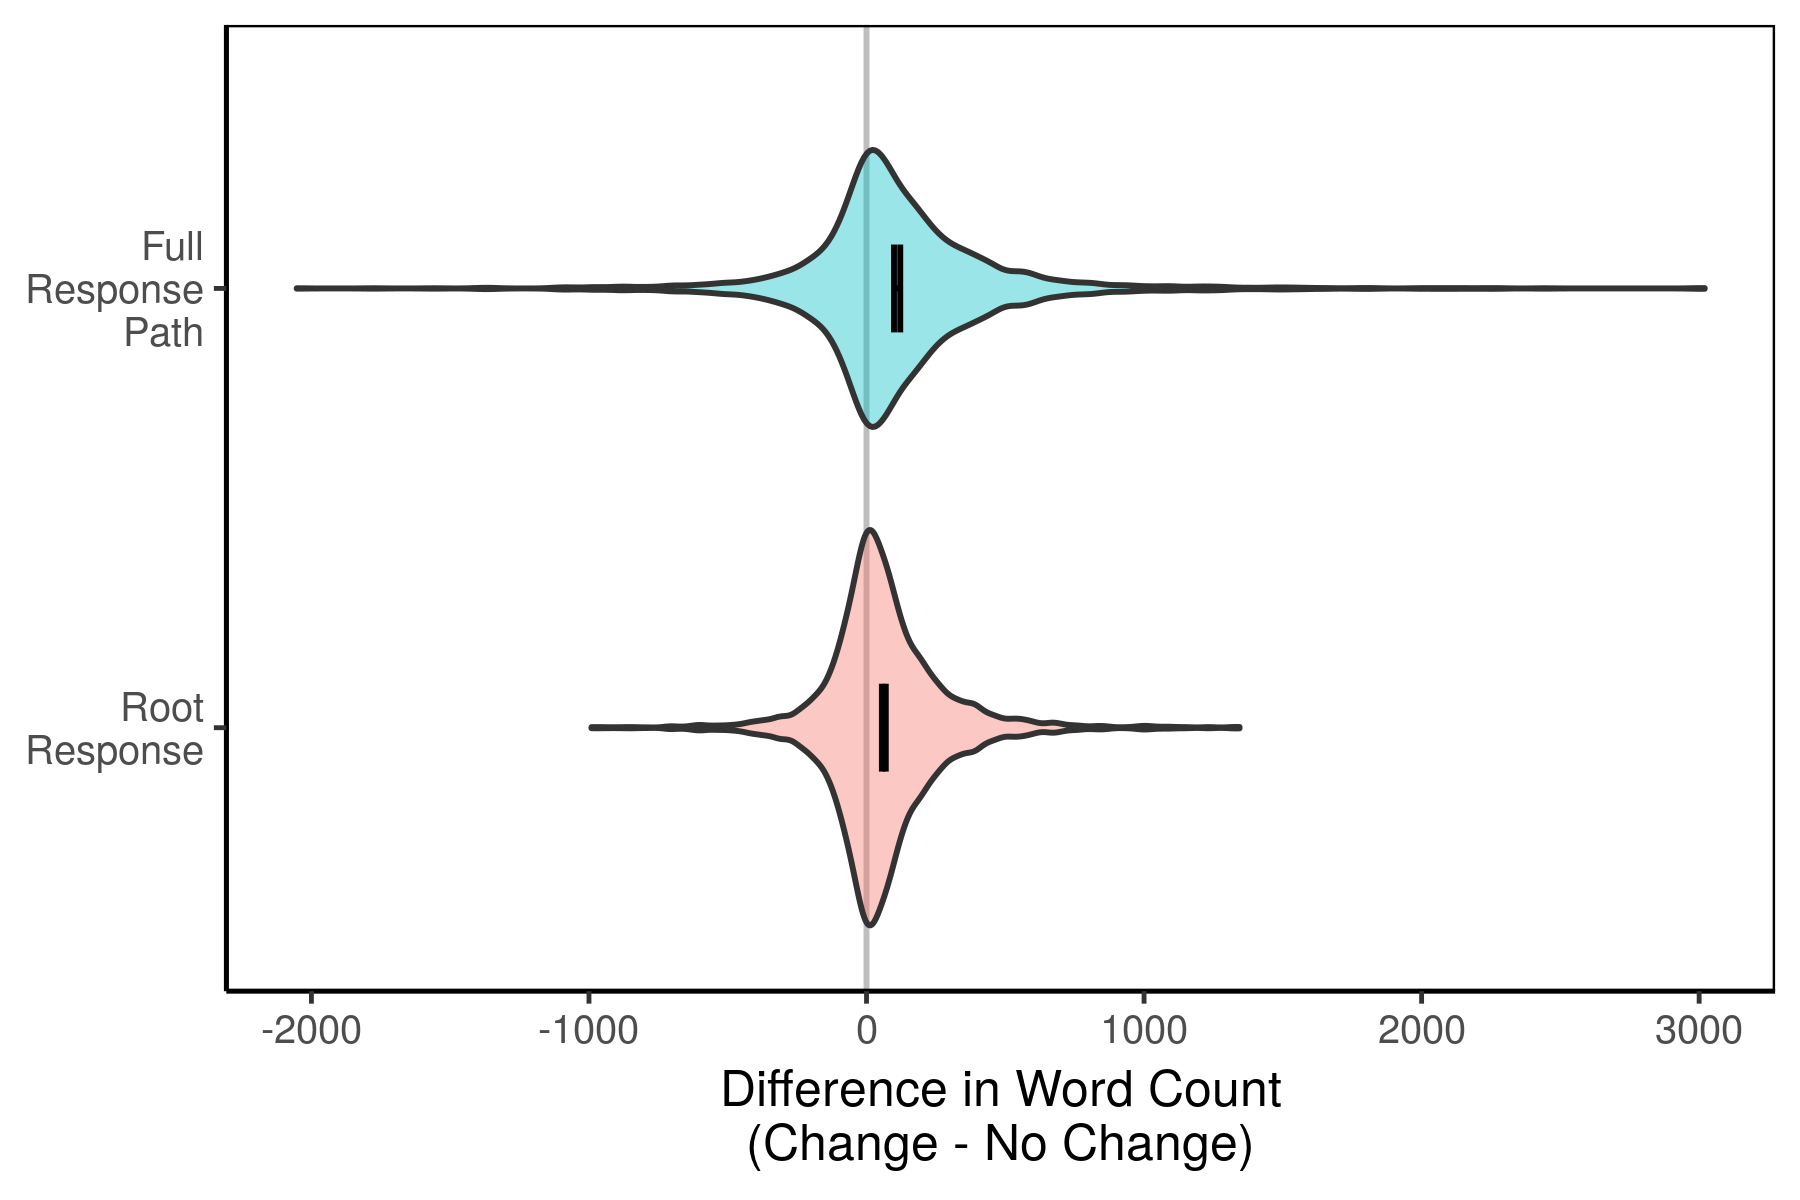
\includegraphics{../calc/fig/wordcount_violin.png}
\end{figure}
\end{frame}

\section{Topic Differences in Persuadability}
\begin{frame}{Topic Differences in Persuadability}
\begin{figure}
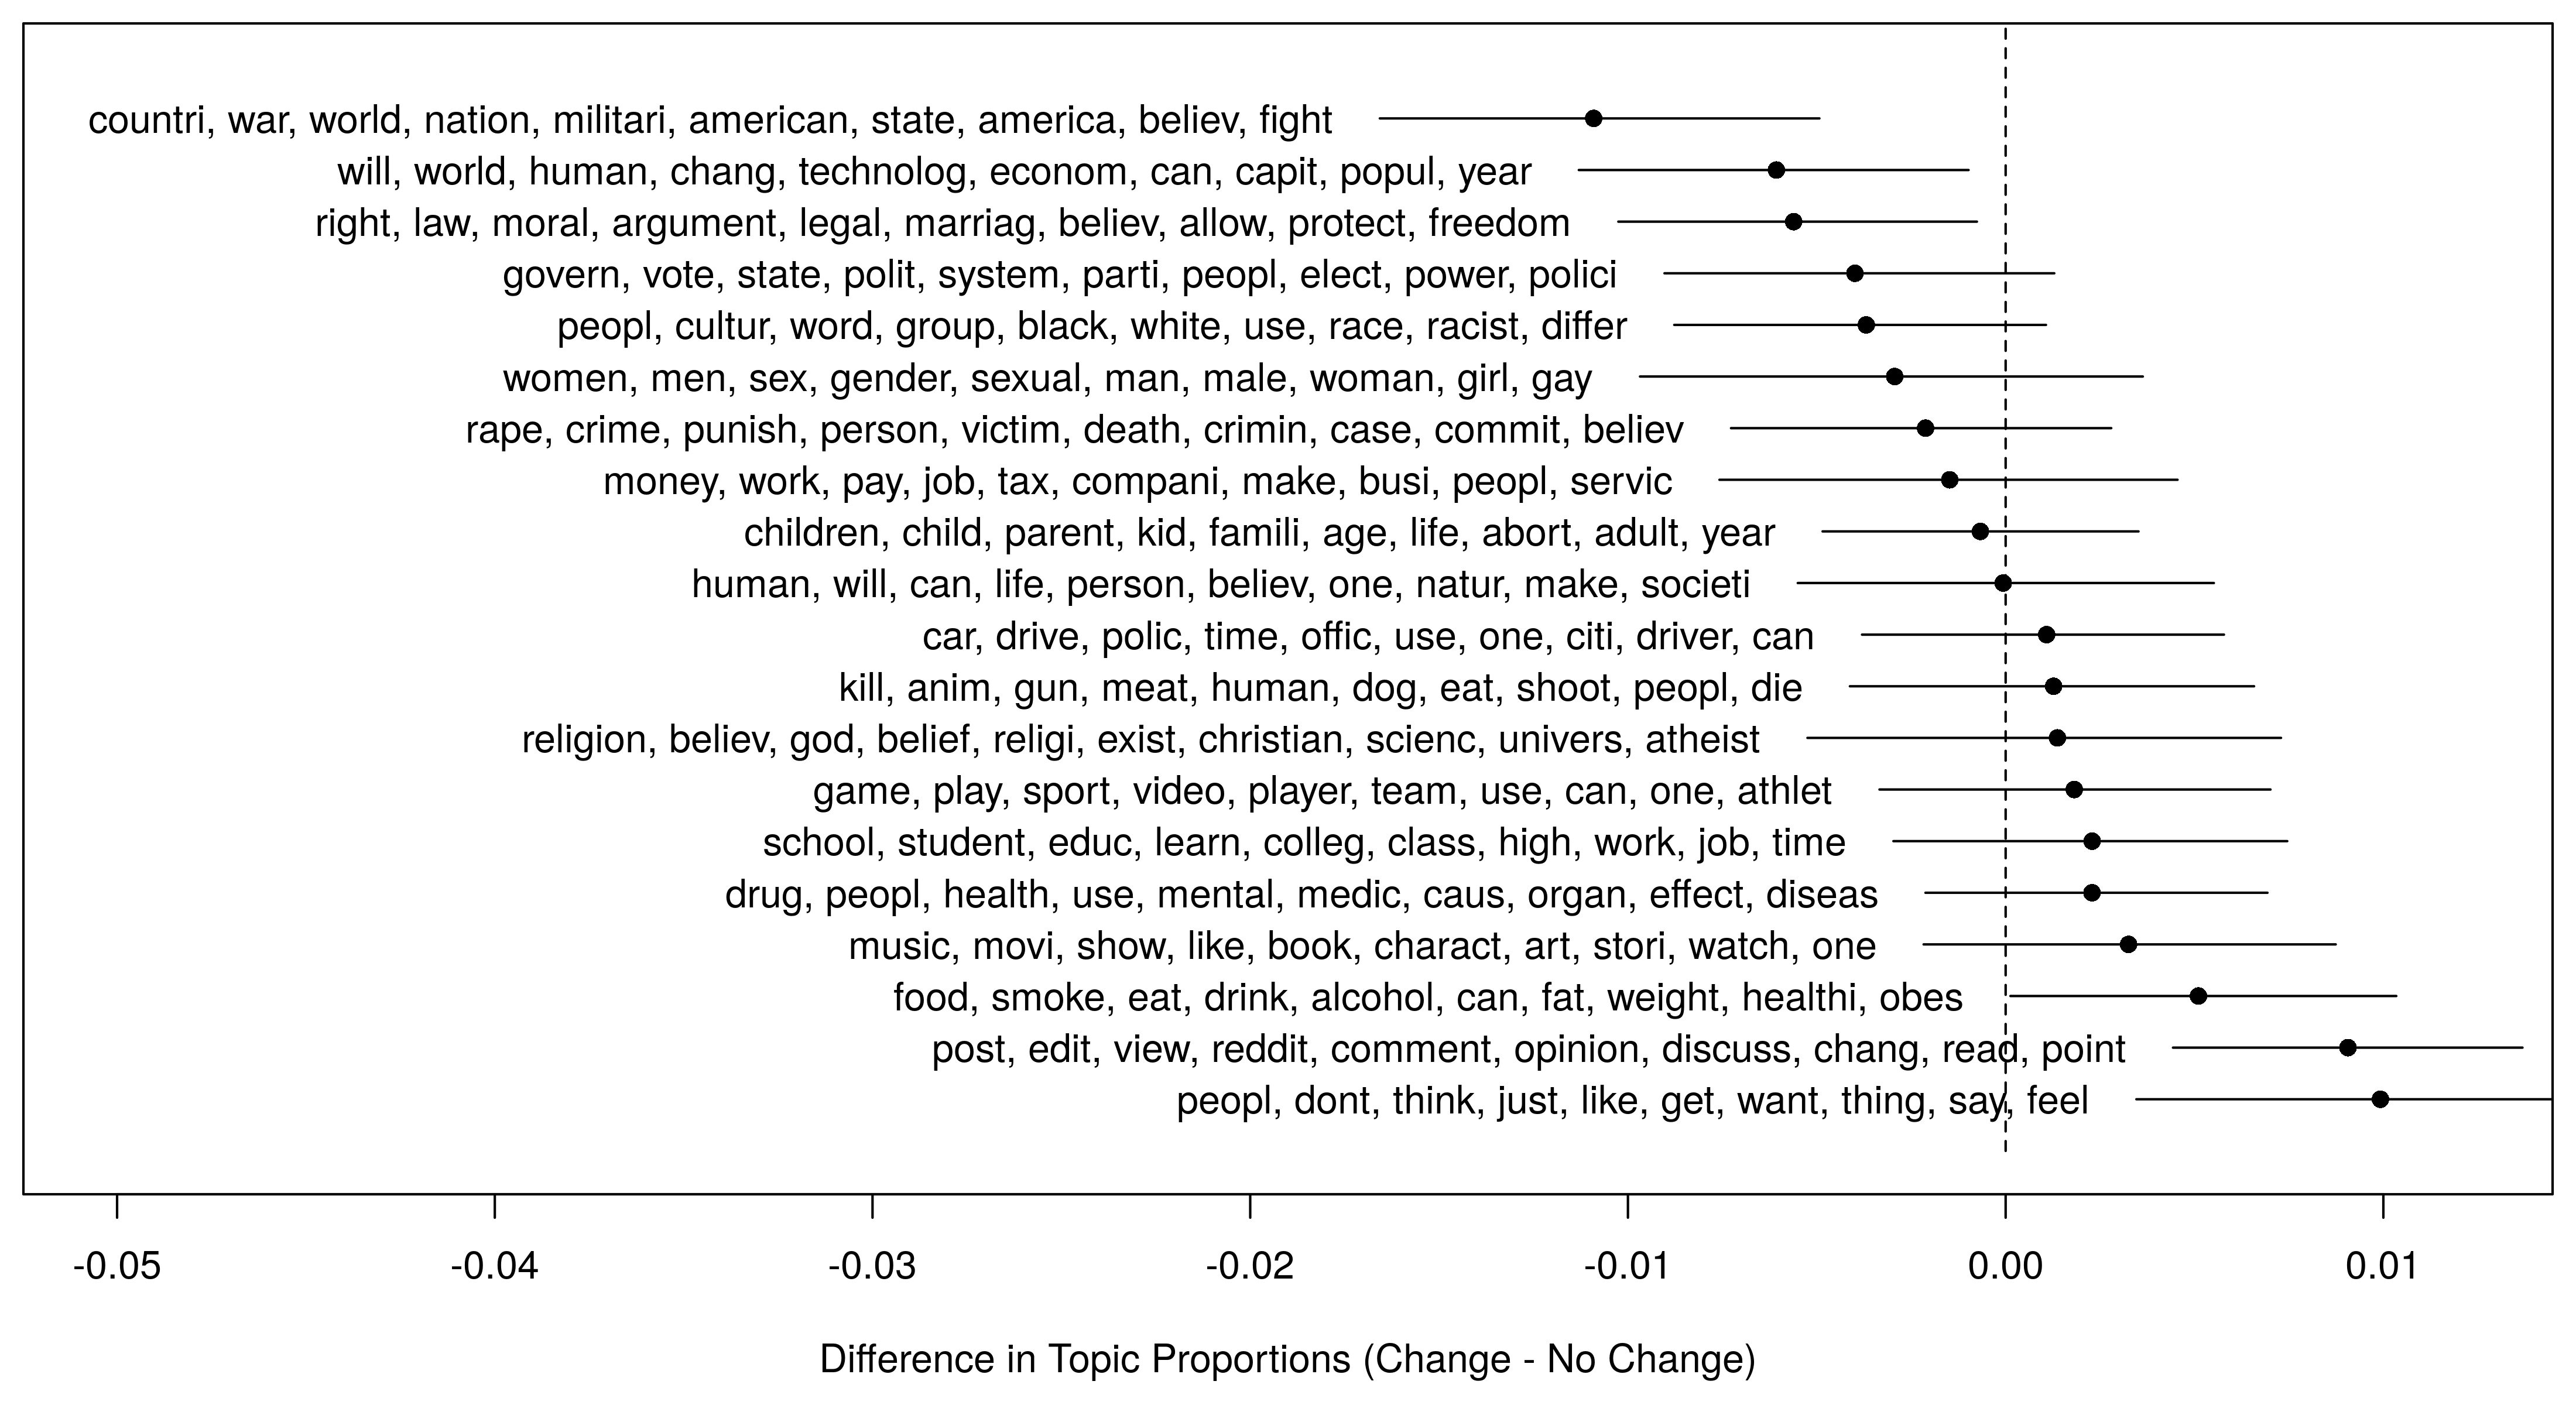
\includegraphics[width=\textwidth]{../calc/fig/stm_op_diff.png}
\end{figure}
\end{frame}

\begin{frame} %<beamer:0> % hide references
  \frametitle{References}
  \def\newblock{\hskip .11em plus .33em minus .07em}
  %\nocite{*}
  \begin{scriptsize}
    \bibliographystyle{/data/Dropbox/Uni/Lit/apsr2006}
    \bibliography{/data/Dropbox/Uni/Lit/Literature}
  \end{scriptsize}
\end{frame}

\end{document}